\documentclass[11pt,a4paper]{article}

\usepackage[T1]{fontenc}
\usepackage[utf8]{inputenc}
\usepackage{lmodern}
\usepackage{amsmath,amssymb,bm,mathtools}
\usepackage{geometry}
\usepackage{booktabs,array,longtable}
\usepackage{graphicx}
\usepackage{hyperref}
\geometry{margin=2.3cm}
\setlength{\parindent}{0pt}
\setlength{\parskip}{4pt}
\allowdisplaybreaks

\newcommand{\Div}{\operatorname{div}}
\newcommand{\Grad}{\operatorname{grad}}
\newcommand{\dd}{\mathrm{d}}
\newcommand{\Id}{\mathbf I}

\title{Formula\c{c}\~ao poroel\'astica n\~ao saturada\\
\large Esqueleto deform\'avel, \`agua e ar\\[2pt]
\normalsize Vers\~ao 4: implementa\c{c}\~ao no NeoPZ, reprodu\c{c}\~ao de Rahardjo et al.\ (2007) e dire\c{c}\~oes de investiga\c{c}\~ao}
\author{}
\date{}

\begin{document}
\maketitle
\vspace{-2em}

\section{Hip\'oteses e vari\'aveis prim\'arias}

Consideram-se pequenas deforma\c{c}\~oes, regime quase est\'atico,
temperatura constante, esqueleto el\'astico isot\'ropo e duas fases fluidas
(\'agua e ar) sem mudan\c{c}a de fase. O escoamento de cada fase segue
a lei de Darcy generalizada com permeabilidade relativa. A contribui\c{c}\~ao
das press\~oes \`a tens\~ao total utiliza a hip\'otese de Bishop
$\chi=S_w$; trata-se de uma escolha constitutiva, n\~ao de uma identidade
universal para todos os solos.

As vari\'aveis prim\'arias s\~ao
\begin{equation*}
\boxed{\mathbf u(\mathbf x,t),\qquad p_w(\mathbf x,t),\qquad p_a(\mathbf x,t).}
\end{equation*}
Para explicitar as depend\^encias funcionais, define-se
\begin{equation*}
\mathbf z=(\mathbf u,p_w,p_a),\qquad
n(\mathbf z)=n(\mathbf u,p_w,p_a),\qquad
\alpha(n(\mathbf z))=\alpha\bigl(n(\mathbf u,p_w,p_a)\bigr).
\end{equation*}
As derivadas temporais das grandezas materiais s\~ao tomadas acompanhando
o movimento do esqueleto s\'olido. No contexto de pequenas deforma\c{c}\~oes,
usa-se o ponto para essa derivada.

\section{Cinem\'atica e constantes el\'asticas}

\begin{equation*}
\boxed{\boldsymbol\varepsilon(\mathbf u)=
\frac12\left[\nabla\mathbf u+(\nabla\mathbf u)^{\mathsf T}\right],
\qquad \varepsilon_v(\mathbf u)=\Div\mathbf u.}
\end{equation*}
\begin{equation*}
G=\frac{E_d}{2(1+\nu_d)},\qquad
\lambda=\frac{E_d\nu_d}{(1+\nu_d)(1-2\nu_d)},\qquad
K_d=\frac{E_d}{3(1-2\nu_d)}.
\end{equation*}
\begin{equation*}
\boxed{\alpha(n(\mathbf z))=1-\frac{K_d(n(\mathbf z))}{K_s}.}
\end{equation*}
Na aproxima\c{c}\~ao el\'astica linear de refer\^encia, $E_d$, $\nu_d$
e $\alpha=\alpha_0$ podem ser mantidos constantes. A depend\^encia de
$K_d$ com $n(\mathbf z)$ requer calibra\c{c}\~ao experimental adicional.

\section{Suc\c{c}\~ao, satura\c{c}\~ao e press\~ao equivalente}

\begin{equation*}
\boxed{p_c(p_w,p_a)=p_a-p_w.}
\end{equation*}
\begin{equation*}
\boxed{S_w(p_w,p_a)=S_w\bigl(p_c(p_w,p_a)\bigr),\qquad
S_a(p_w,p_a)=1-S_w(p_w,p_a).}
\end{equation*}
\begin{equation*}
\boxed{p_B(p_w,p_a)=S_w(p_w,p_a)p_w+S_a(p_w,p_a)p_a
=p_a-S_w(p_w,p_a)p_c(p_w,p_a).}
\end{equation*}

Como parametriza\c{c}\~ao experimental da reten\c{c}\~ao, pode-se empregar
van Genuchten, para $p_c(p_w,p_a)>0$:
\begin{align*}
m_{\mathrm{VG}}&=1-\frac{1}{b_{\mathrm{VG}}},\\
S_e(p_w,p_a)&=\left[1+\left(a_{\mathrm{VG}}p_c(p_w,p_a)\right)^{b_{\mathrm{VG}}}\right]^{-m_{\mathrm{VG}}},\\
\boxed{S_w(p_w,p_a)}&\boxed{=S_{wr}+(1-S_{wr})S_e(p_w,p_a).}
\end{align*}
Para $p_c(p_w,p_a)\leq0$, adota-se $S_w(p_w,p_a)=1$ e
$S_a(p_w,p_a)=0$. Histerese de secagem e umedecimento n\~ao est\'a
inclu\'ida nesta primeira formula\c{c}\~ao.

Para reten\c{c}\~ao independente de $n(\mathbf z)$, define-se
\begin{equation*}
\boxed{\Gamma(p_w,p_a)=\frac{\partial S_w(p_w,p_a)}{\partial p_w}
=-\frac{\partial S_w(p_w,p_a)}{\partial p_a}.}
\end{equation*}
No ramo n\~ao saturado de van Genuchten:
\begin{equation*}
\Gamma(p_w,p_a)=(1-S_{wr})m_{\mathrm{VG}}b_{\mathrm{VG}}
a_{\mathrm{VG}}^{b_{\mathrm{VG}}}
[p_c(p_w,p_a)]^{b_{\mathrm{VG}}-1}
\left[1+\left(a_{\mathrm{VG}}p_c(p_w,p_a)\right)^{b_{\mathrm{VG}}}\right]^{-m_{\mathrm{VG}}-1}.
\end{equation*}

\section{Equil\'ibrio mec\^anico do esqueleto}\label{sec:equilibrio}

Com a conven\c{c}\~ao de tens\~oes positivas em tra\c{c}\~ao,
\begin{equation*}
\boxed{\Div\boldsymbol\sigma(\mathbf z)+\rho_b(\mathbf z)\mathbf g=\mathbf0.}
\end{equation*}
A tens\~ao total incremental, relativa ao estado inicial, \`e
\begin{equation*}
\boxed{\begin{aligned}
\boldsymbol\sigma(\mathbf z)={}&\boldsymbol\sigma_0
+2G\boldsymbol\varepsilon(\mathbf u)
+\lambda\varepsilon_v(\mathbf u)\Id\\
&-\alpha(n(\mathbf z))
\left[p_B(p_w,p_a)-p_{B0}\right]\Id.
\end{aligned}}
\end{equation*}
Com $\rho_s$ representando a massa espec\'ifica dos gr\~aos,
\begin{equation*}
\boxed{\begin{aligned}
\rho_b(\mathbf z)={}&[1-n(\mathbf z)]\rho_s\\
&+n(\mathbf z)\left[
S_w(p_w,p_a)\rho_w(p_w)+S_a(p_w,p_a)\rho_a(p_a)
\right].
\end{aligned}}
\end{equation*}
O tensor $\boldsymbol\sigma_0$ representa o estado de tens\~oes inicial;
o termo $p_{B0}$ \`e a press\~ao equivalente nesse mesmo estado.

\section{Leis de Darcy para as duas fases}

\begin{equation*}
\boxed{\mathbf q_w(\mathbf z)=
-\frac{\kappa(n(\mathbf z))k_{rw}(S_w(p_w,p_a))}{\mu_w}
\left[\nabla p_w-\rho_w(p_w)\mathbf g\right].}
\end{equation*}
\begin{equation*}
\boxed{\mathbf q_a(\mathbf z)=
-\frac{\kappa(n(\mathbf z))k_{ra}(S_a(p_w,p_a))}{\mu_a}
\left[\nabla p_a-\rho_a(p_a)\mathbf g\right].}
\end{equation*}
Os fluxos $\mathbf q_w(\mathbf z)$ e $\mathbf q_a(\mathbf z)$ s\~ao
velocidades superficiais relativas ao esqueleto, em $\mathrm{m/s}$.

Uma rela\c{c}\~ao de Kozeny--Carman para a varia\c{c}\~ao da
permeabilidade intr\'inseca \`e
\begin{equation*}
\boxed{\kappa(n(\mathbf z))=\kappa_0
\left(\frac{n(\mathbf z)}{n_0}\right)^3
\left(\frac{1-n_0}{1-n(\mathbf z)}\right)^2.}
\end{equation*}
Para as permeabilidades relativas, uma escolha Mualem--van Genuchten \`e
\begin{equation*}
\boxed{\begin{aligned}
k_{rw}(S_w(p_w,p_a))={}&[S_e(p_w,p_a)]^{1/2}
\left\{1-\left[1-[S_e(p_w,p_a)]^{1/m_{\mathrm{VG}}}\right]^{m_{\mathrm{VG}}}\right\}^{2},\\
k_{ra}(S_a(p_w,p_a))={}&[1-S_e(p_w,p_a)]^{1/2}
\left[1-[S_e(p_w,p_a)]^{1/m_{\mathrm{VG}}}\right]^{2m_{\mathrm{VG}}}.
\end{aligned}}
\end{equation*}
Essas duas curvas devem ser verificadas experimentalmente, sobretudo na
presen\c{c}a de ar aprisionado ou satura\c{c}\~ao residual de g\'as.

\section{Compressibilidade e massa espec\'ifica dos fluidos}\label{sec:fluidos}

Com $K_w$ constante,
\begin{equation*}
\boxed{\rho_w(p_w)=\rho_{w0}
\exp\left(\frac{p_w-p_{w0}}{K_w}\right).}
\end{equation*}
Para ar ideal isot\'ermico,
\begin{equation*}
\boxed{\rho_a(p_a)=\rho_{a0}\frac{p_a^{\mathrm{abs}}}{p_{a0}^{\mathrm{abs}}},
\qquad K_a(p_a)=p_a^{\mathrm{abs}}.}
\end{equation*}
As press\~oes usadas na equa\c{c}\~ao de estado do ar s\~ao absolutas;
as diferen\c{c}as de press\~ao na suc\c{c}\~ao independem da escolha de
refer\^encia manom\'etrica. As viscosidades $\mu_w$ e $\mu_a$ podem ser
consideradas constantes a temperatura fixa.

\section{Armazenamento e acoplamento entre as fases}

Para escrever as equa\c{c}\~oes com coeficientes dependentes do estado,
definem-se
\begin{equation*}
\boxed{\eta(\mathbf z)=\frac{\alpha(n(\mathbf z))-n(\mathbf z)}{K_s}.}
\end{equation*}
\begin{equation*}
\boxed{\begin{aligned}
D_w(\mathbf z)&=n(\mathbf z)-\eta(\mathbf z)S_w(p_w,p_a)p_c(p_w,p_a),\\
D_a(\mathbf z)&=-n(\mathbf z)-\eta(\mathbf z)S_a(p_w,p_a)p_c(p_w,p_a).
\end{aligned}}
\end{equation*}

Os coeficientes associados \`a deforma\c{c}\~ao volum\'etrica s\~ao
\begin{equation*}
\boxed{\begin{aligned}
B_w(\mathbf z)&=\alpha(n(\mathbf z))S_w(p_w,p_a),\\
B_a(\mathbf z)&=\alpha(n(\mathbf z))S_a(p_w,p_a).
\end{aligned}}
\end{equation*}

Os quatro coeficientes de armazenamento s\~ao
\begin{equation*}
\boxed{\begin{aligned}
C_{ww}(\mathbf z)={}&\eta(\mathbf z)[S_w(p_w,p_a)]^2
+\frac{n(\mathbf z)S_w(p_w,p_a)}{K_w}
+D_w(\mathbf z)\Gamma(p_w,p_a),\\
C_{wa}(\mathbf z)={}&\eta(\mathbf z)S_w(p_w,p_a)S_a(p_w,p_a)
-D_w(\mathbf z)\Gamma(p_w,p_a),\\
C_{aw}(\mathbf z)={}&\eta(\mathbf z)S_a(p_w,p_a)S_w(p_w,p_a)
+D_a(\mathbf z)\Gamma(p_w,p_a),\\
C_{aa}(\mathbf z)={}&\eta(\mathbf z)[S_a(p_w,p_a)]^2
+\frac{n(\mathbf z)S_a(p_w,p_a)}{K_a(p_a)}
-D_a(\mathbf z)\Gamma(p_w,p_a).
\end{aligned}}
\end{equation*}

Essas express\~oes decorrem da forma incremental do conte\'udo de cada
fase, para o modelo poroel\'astico adotado:
\begin{equation*}
\dot\zeta_i=S_i\left[\alpha\dot\varepsilon_v+\eta\dot p_B\right]
+n\dot S_i+\frac{nS_i}{K_i}\dot p_i,
\qquad i\in\{w,a\},
\end{equation*}
com $S_a=1-S_w$ e $\dot p_B=S_w\dot p_w+S_a\dot p_a
+(p_w-p_a)\dot S_w$. Nessa \'ultima express\~ao, os coeficientes
s\~ao tangentes avaliados no estado atual, e n\~ao derivadas de produtos
de coeficientes secantes com incrementos acumulados.

\section{Equa\c{c}\~oes de Biot para difus\~ao da \`agua e do ar}

A conserva\c{c}\~ao da massa de cada fase, em forma normalizada pela
massa espec\'ifica, fornece
\begin{equation*}
\boxed{\begin{aligned}
B_w(\mathbf z)\frac{\partial\varepsilon_v(\mathbf u)}{\partial t}
&+C_{ww}(\mathbf z)\frac{\partial p_w}{\partial t}
+C_{wa}(\mathbf z)\frac{\partial p_a}{\partial t}\\
&+\frac{1}{\rho_w(p_w)}\Div\left[\rho_w(p_w)\mathbf q_w(\mathbf z)\right]=s_w.
\end{aligned}}
\end{equation*}
\begin{equation*}
\boxed{\begin{aligned}
B_a(\mathbf z)\frac{\partial\varepsilon_v(\mathbf u)}{\partial t}
&+C_{aw}(\mathbf z)\frac{\partial p_w}{\partial t}
+C_{aa}(\mathbf z)\frac{\partial p_a}{\partial t}\\
&+\frac{1}{\rho_a(p_a)}\Div\left[\rho_a(p_a)\mathbf q_a(\mathbf z)\right]=s_a.
\end{aligned}}
\end{equation*}
Os termos $s_w$ e $s_a$ representam fontes de massa de fase divididas
pela massa espec\'ifica correspondente (unidade $\mathrm{s}^{-1}$).

\section{Fechamento da porosidade}

Uma aproxima\c{c}\~ao poroel\'astica linearizada em torno do estado
inicial, consistente com a forma saturada de Biot, \`e
\begin{equation*}
\boxed{\begin{aligned}
n(\mathbf z)={}&n_0+(\alpha_0-n_0)\varepsilon_v(\mathbf u)\\
&+\frac{\alpha_0-n_0}{K_s}
\left[p_B(p_w,p_a)-p_{B0}\right].
\end{aligned}}
\end{equation*}
Esse fechamento \`e v\'alido em primeira ordem, com $\alpha_0$ medido
no estado de refer\^encia. Para varia\c{c}\~oes materiais expressivas,
deve ser substitu\'ido por uma lei de evolu\c{c}\~ao da porosidade
calibrada em ensaios de compressibilidade e trajet\'orias de suc\c{c}\~ao.

\section{Sistema acoplado final}

\begin{equation*}
\boxed{\begin{aligned}
\Div\boldsymbol\sigma(\mathbf z)+\rho_b(\mathbf z)\mathbf g&=\mathbf0,\\[2pt]
B_w(\mathbf z)\dot\varepsilon_v(\mathbf u)
+C_{ww}(\mathbf z)\dot p_w+C_{wa}(\mathbf z)\dot p_a
+\frac{1}{\rho_w(p_w)}\Div[\rho_w(p_w)\mathbf q_w(\mathbf z)]&=s_w,\\[2pt]
B_a(\mathbf z)\dot\varepsilon_v(\mathbf u)
+C_{aw}(\mathbf z)\dot p_w+C_{aa}(\mathbf z)\dot p_a
+\frac{1}{\rho_a(p_a)}\Div[\rho_a(p_a)\mathbf q_a(\mathbf z)]&=s_a.
\end{aligned}}
\end{equation*}
As tr\^es equa\c{c}\~oes s\~ao resolvidas para $\mathbf u$, $p_w$
e $p_a$. A porosidade e as satura\c{c}\~oes n\~ao s\~ao vari\'aveis
prim\'arias independentes: s\~ao calculadas pelas rela\c{c}\~oes
constitutivas declaradas acima.

\section{Extens\~ao: reten\c{c}\~ao dependente da porosidade}

Se a curva de reten\c{c}\~ao depender tamb\'em da porosidade, escreve-se
\begin{equation*}
\boxed{S_w(\mathbf z)=\mathcal S\bigl(p_a-p_w,n(\mathbf z)\bigr),
\qquad S_a(\mathbf z)=1-S_w(\mathbf z).}
\end{equation*}
Nesse caso, todas as ocorr\^encias de $S_w(p_w,p_a)$ e
$S_a(p_w,p_a)$ nas express\~oes anteriores devem ser substitu\'idas
por $S_w(\mathbf z)$ e $S_a(\mathbf z)$. Definem-se as derivadas totais
de estado
\begin{align*}
\Gamma_{\varepsilon}(\mathbf z)
&=\frac{\partial\mathcal S}{\partial n}
\frac{\partial n(\mathbf z)}{\partial\varepsilon_v},\\
\Gamma_w(\mathbf z)
&=-\frac{\partial\mathcal S}{\partial p_c}
+\frac{\partial\mathcal S}{\partial n}
\frac{\partial n(\mathbf z)}{\partial p_w},\\
\Gamma_a(\mathbf z)
&=\frac{\partial\mathcal S}{\partial p_c}
+\frac{\partial\mathcal S}{\partial n}
\frac{\partial n(\mathbf z)}{\partial p_a}.
\end{align*}
Os coeficientes modificados ficam
\begin{equation*}
\boxed{\begin{aligned}
B_w(\mathbf z)&=\alpha(n(\mathbf z))S_w(\mathbf z)
+D_w(\mathbf z)\Gamma_{\varepsilon}(\mathbf z),\\
B_a(\mathbf z)&=\alpha(n(\mathbf z))S_a(\mathbf z)
+D_a(\mathbf z)\Gamma_{\varepsilon}(\mathbf z),\\
C_{ww}(\mathbf z)&=\eta(\mathbf z)[S_w(\mathbf z)]^2
+\frac{n(\mathbf z)S_w(\mathbf z)}{K_w}
+D_w(\mathbf z)\Gamma_w(\mathbf z),\\
C_{wa}(\mathbf z)&=\eta(\mathbf z)S_w(\mathbf z)S_a(\mathbf z)
+D_w(\mathbf z)\Gamma_a(\mathbf z),\\
C_{aw}(\mathbf z)&=\eta(\mathbf z)S_a(\mathbf z)S_w(\mathbf z)
+D_a(\mathbf z)\Gamma_w(\mathbf z),\\
C_{aa}(\mathbf z)&=\eta(\mathbf z)[S_a(\mathbf z)]^2
+\frac{n(\mathbf z)S_a(\mathbf z)}{K_a(p_a)}
+D_a(\mathbf z)\Gamma_a(\mathbf z).
\end{aligned}}
\end{equation*}
Se $n(\mathbf z)$ tamb\'em depender de $S_w(\mathbf z)$ por meio de
$p_B$, o fechamento local \`e impl\'icito e suas derivadas devem ser
calculadas consistentemente (por diferencia\c{c}\~ao impl\'icita).

\section{Verifica\c{c}\~ao do limite saturado}

Para $S_w=1$, $S_a=0$ e derivadas de satura\c{c}\~ao nulas,
\begin{equation*}
B_w=\alpha,\qquad
C_{ww}=\frac{\alpha-n}{K_s}+\frac{n}{K_w}=\frac1M,\qquad
C_{wa}=0.
\end{equation*}
A equa\c{c}\~ao da \`agua recupera
\begin{equation*}
\boxed{\alpha\frac{\partial}{\partial t}(\Div\mathbf u)
+\frac1M\frac{\partial p_w}{\partial t}
-\Div\left[\frac{\kappa(n)}{\mu_w}
(\nabla p_w-\rho_w\mathbf g)\right]=s_w,}
\end{equation*}
na aproxima\c{c}\~ao de pequena varia\c{c}\~ao espacial de
$\rho_w$. Quando $S_a\to0$, a press\~ao do ar deixa de ser uma vari\'avel
independente fisicamente definida: a implementa\c{c}\~ao deve tratar
o desaparecimento da fase gasosa.

\section{Discretização por elementos finitos}

\subsection{Problema de valor de contorno}

Seja $\Omega\subset\mathbb R^{2}$ (estado plano de deformação, espessura
unitária) com contorno $\Gamma$. Para cada campo, o contorno se divide em
partes de Dirichlet e de Neumann:
\begin{equation*}
\Gamma=\Gamma_u\cup\Gamma_t,\qquad
\Gamma=\Gamma_p^{\pi}\cup\Gamma_q^{\pi},\qquad \pi\in\{w,a\},
\end{equation*}
\begin{equation*}
\boxed{\begin{aligned}
\mathbf u&=\bar{\mathbf u}\ \text{em}\ \Gamma_u, &
\boldsymbol\sigma\mathbf n&=\bar{\mathbf t}\ \text{em}\ \Gamma_t,\\
p_\pi&=\bar p_\pi\ \text{em}\ \Gamma_p^{\pi}, &
\mathbf q_\pi\cdot\mathbf n&=\bar q_\pi\ \text{em}\ \Gamma_q^{\pi},
\end{aligned}}
\end{equation*}
com $\mathbf n$ normal unitária externa e $\bar q_\pi>0$ indicando saída
de fluido. As condições iniciais são $\mathbf u(\mathbf x,0)=\mathbf u_0$,
$p_\pi(\mathbf x,0)=p_{\pi0}$, compatíveis com $\boldsymbol\sigma_0$ e
$p_{B0}$.

\subsection{Forma fraca}

Sejam as funções-teste $\mathbf v\in\mathcal V_u$ e $w\in\mathcal V_p$,
nulas em $\Gamma_u$ e $\Gamma_p^{\pi}$, respectivamente.

\paragraph{Equilíbrio.} Multiplicando por $\mathbf v$ e integrando por partes:
\begin{equation*}
\boxed{\int_\Omega\boldsymbol\varepsilon(\mathbf v):\boldsymbol\sigma(\mathbf z)\,\dd\Omega
=\int_\Omega\mathbf v\cdot\rho_b(\mathbf z)\mathbf g\,\dd\Omega
+\int_{\Gamma_t}\mathbf v\cdot\bar{\mathbf t}\,\dd\Gamma.}
\end{equation*}

\paragraph{Fases fluidas.} O termo de transporte é expandido como
\begin{equation*}
\frac{1}{\rho_\pi}\Div(\rho_\pi\mathbf q_\pi)
=\Div\mathbf q_\pi+c_\pi\,\mathbf q_\pi\cdot\nabla p_\pi,
\qquad
c_\pi=\frac{1}{\rho_\pi}\frac{\dd\rho_\pi}{\dd p_\pi},
\end{equation*}
o que, pelas equações de estado da Seção~\ref{sec:fluidos}, dá
\begin{equation*}
c_w=\frac{1}{K_w},\qquad c_a(p_a)=\frac{1}{p_a^{\mathrm{abs}}}.
\end{equation*}
Integrando $\Div\mathbf q_\pi$ por partes, obtém-se, para $\pi\in\{w,a\}$:
\begin{equation*}
\boxed{\begin{aligned}
&\int_\Omega w\left[B_\pi\dot\varepsilon_v+C_{\pi w}\dot p_w+C_{\pi a}\dot p_a\right]\dd\Omega
-\int_\Omega\nabla w\cdot\mathbf q_\pi\,\dd\Omega
+\int_\Omega w\,c_\pi\,\mathbf q_\pi\cdot\nabla p_\pi\,\dd\Omega\\
&\qquad=\int_\Omega w\,s_\pi\,\dd\Omega-\int_{\Gamma_q^{\pi}}w\,\bar q_\pi\,\dd\Gamma .
\end{aligned}}
\end{equation*}
Com a lei de Darcy, $-\nabla w\cdot\mathbf q_\pi
=\nabla w\cdot\lambda_\pi(\nabla p_\pi-\rho_\pi\mathbf g)$, em que
\begin{equation*}
\boxed{\lambda_\pi(\mathbf z)=\frac{\kappa(n(\mathbf z))\,k_{r\pi}(S_\pi)}{\mu_\pi}
\qquad[\mathrm{m^2/(Pa\,s)}].}
\end{equation*}

\subsection{Aproximação espacial (Galerkin)}

Em cada elemento $\Omega^e$, com $n_e$ nós,
\begin{equation*}
\boxed{\mathbf u\approx\mathbf N_u\mathbf U^e,\qquad
p_w\approx\mathbf N_p\mathbf P_w^e,\qquad
p_a\approx\mathbf N_p\mathbf P_a^e,}
\end{equation*}
\begin{equation*}
\boxed{\boldsymbol\varepsilon\approx\mathbf B_u\mathbf U^e,\qquad
\varepsilon_v\approx\mathbf m^{\mathsf T}\mathbf B_u\mathbf U^e,\qquad
\nabla p_\pi\approx\mathbf B_p\mathbf P_\pi^e.}
\end{equation*}
Usa-se notação de Voigt em estado plano de deformação:
\begin{equation*}
\boldsymbol\varepsilon=\begin{Bmatrix}\varepsilon_{xx}\\ \varepsilon_{yy}\\ \gamma_{xy}\end{Bmatrix},
\qquad
\boldsymbol\sigma=\begin{Bmatrix}\sigma_{xx}\\ \sigma_{yy}\\ \sigma_{xy}\end{Bmatrix},
\qquad
\mathbf m=\begin{Bmatrix}1\\1\\0\end{Bmatrix},
\qquad
\mathbf D_e=\begin{bmatrix}\lambda+2G&\lambda&0\\ \lambda&\lambda+2G&0\\ 0&0&G\end{bmatrix}.
\end{equation*}
A lei constitutiva da Seção~\ref{sec:equilibrio} fica
\begin{equation*}
\boxed{\boldsymbol\sigma(\mathbf z)=\boldsymbol\sigma_0+\mathbf D_e\mathbf B_u\mathbf U^e
-\alpha(n(\mathbf z))\left[p_B(p_w,p_a)-p_{B0}\right]\mathbf m,}
\end{equation*}
e, se necessário, $\sigma_{zz}=\sigma_{zz,0}+\lambda\varepsilon_v-\alpha(p_B-p_{B0})$
é recuperada no pós-processamento. A forma explícita de $\mathbf N_u$,
$\mathbf B_u$, $\mathbf N_p$ e $\mathbf B_p$ para os elementos Q4 e T3
é dada na Seção~\ref{sec:matrizes}.

Os vetores globais $\mathbf U$, $\mathbf P_w$ e $\mathbf P_a$ são obtidos
pela montagem $\mathsf A_e$ das contribuições elementares, e
\begin{equation*}
\mathbf X=\begin{Bmatrix}\mathbf U\\ \mathbf P_w\\ \mathbf P_a\end{Bmatrix}.
\end{equation*}

\subsection{Matrizes e vetores elementares}

Os coeficientes são avaliados nos pontos de integração, no estado atual.
\begin{center}
\renewcommand{\arraystretch}{1.6}
\begin{tabular}{p{0.30\linewidth}p{0.55\linewidth}}
\toprule
Grandeza & Definição\\
\midrule
Rigidez tangente &
$\mathbf K=\displaystyle\int_{\Omega^e}\mathbf B_u^{\mathsf T}\mathbf D_T\mathbf B_u\,\dd\Omega$\\
Acoplamento $\mathbf u\leftarrow p_\pi$ &
$\mathbf Q_{u\pi}=\displaystyle\int_{\Omega^e}\mathbf B_u^{\mathsf T}\mathbf m\,\alpha\,\chi_\pi\,\mathbf N_p\,\dd\Omega$\\
Acoplamento $p_\pi\leftarrow\mathbf u$ &
$\mathbf Q_{\pi u}=\displaystyle\int_{\Omega^e}\mathbf N_p^{\mathsf T}B_\pi\,\mathbf m^{\mathsf T}\mathbf B_u\,\dd\Omega$\\
Armazenamento &
$\mathbf C_{\pi\beta}=\displaystyle\int_{\Omega^e}\mathbf N_p^{\mathsf T}C_{\pi\beta}\mathbf N_p\,\dd\Omega$,\quad $\pi,\beta\in\{w,a\}$\\
Condução (Darcy) &
$\mathbf H_\pi=\displaystyle\int_{\Omega^e}\mathbf B_p^{\mathsf T}\lambda_\pi\mathbf B_p\,\dd\Omega$\\
\bottomrule
\end{tabular}
\end{center}

Nessas expressões, $\chi_\pi=\partial p_B/\partial p_\pi$ são os
coeficientes de Bishop \emph{tangentes}:
\begin{equation*}
\boxed{\chi_w=S_w-\Gamma\,p_c,\qquad \chi_a=S_a+\Gamma\,p_c,\qquad \chi_w+\chi_a=1,}
\end{equation*}
e a matriz constitutiva tangente é
\begin{equation*}
\mathbf D_T=\mathbf D_e-(p_B-p_{B0})\,\frac{\dd\alpha}{\dd n}\frac{\partial n}{\partial\varepsilon_v}\,\mathbf m\mathbf m^{\mathsf T},
\end{equation*}
que se reduz a $\mathbf D_e$ quando $\alpha=\alpha_0$ é constante.
Como $B_\pi=\alpha S_\pi\neq\alpha\chi_\pi$ quando $\Gamma p_c\neq0$,
o acoplamento é em geral não simétrico ($\mathbf Q_{\pi u}\neq\mathbf Q_{u\pi}^{\mathsf T}$);
a simetria é recuperada no limite saturado.

Os vetores de forças são
\begin{align*}
\mathbf f_u&=\int_{\Omega^e}\mathbf N_u^{\mathsf T}\rho_b(\mathbf z)\mathbf g\,\dd\Omega
+\int_{\Gamma_t^e}\mathbf N_u^{\mathsf T}\bar{\mathbf t}\,\dd\Gamma,\\
\mathbf f_\pi&=\int_{\Omega^e}\mathbf N_p^{\mathsf T}s_\pi\,\dd\Omega
+\int_{\Omega^e}\mathbf B_p^{\mathsf T}\lambda_\pi\rho_\pi\mathbf g\,\dd\Omega
-\int_{\Gamma_q^{\pi,e}}\mathbf N_p^{\mathsf T}\bar q_\pi\,\dd\Gamma,
\end{align*}
e o termo de variação espacial da massa específica é
\begin{equation*}
\mathbf g_\pi=\int_{\Omega^e}\mathbf N_p^{\mathsf T}c_\pi\,\mathbf q_\pi\cdot\nabla p_\pi\,\dd\Omega
=-\int_{\Omega^e}\mathbf N_p^{\mathsf T}c_\pi\lambda_\pi
(\mathbf B_p\mathbf P_\pi-\rho_\pi\mathbf g)^{\mathsf T}\mathbf B_p\mathbf P_\pi\,\dd\Omega .
\end{equation*}
Para a água, $c_w=1/K_w$ é tão pequeno que $\mathbf g_w$ costuma ser
desprezado; para o ar, $\mathbf g_a$ deve ser mantido.

\subsection{Sistema semidiscreto}

Em forma de taxas (derivando o equilíbrio no tempo, com coeficientes
congelados), o sistema global é
\begin{equation*}
\boxed{
\begin{bmatrix}\mathbf K&-\mathbf Q_{uw}&-\mathbf Q_{ua}\\
\mathbf Q_{wu}&\mathbf C_{ww}&\mathbf C_{wa}\\
\mathbf Q_{au}&\mathbf C_{aw}&\mathbf C_{aa}\end{bmatrix}
\begin{Bmatrix}\dot{\mathbf U}\\ \dot{\mathbf P}_w\\ \dot{\mathbf P}_a\end{Bmatrix}
+\begin{bmatrix}\mathbf 0&\mathbf 0&\mathbf 0\\ \mathbf 0&\mathbf H_w&\mathbf 0\\ \mathbf 0&\mathbf 0&\mathbf H_a\end{bmatrix}
\begin{Bmatrix}\mathbf U\\ \mathbf P_w\\ \mathbf P_a\end{Bmatrix}
=\begin{Bmatrix}\dot{\mathbf f}_u\\ \mathbf f_w-\mathbf g_w\\ \mathbf f_a-\mathbf g_a\end{Bmatrix}.}
\end{equation*}
De forma compacta, $\mathbf A\dot{\mathbf X}+\mathbf H\mathbf X=\mathbf F$.

\subsection{Discretização temporal}

Com o método $\theta$ ($\tfrac12\leq\theta\leq1$; recomenda-se $\theta=1$,
Euler implícito, por robustez em problemas não saturados), para um passo
$\Delta t=t_{n+1}-t_n$ e coeficientes constantes no passo:
\begin{equation*}
\boxed{\left(\mathbf A+\theta\Delta t\,\mathbf H\right)\Delta\mathbf X
=\begin{Bmatrix}\Delta\mathbf f_u\\ \Delta t\,(\mathbf f_w-\mathbf g_w)^{n+\theta}\\ \Delta t\,(\mathbf f_a-\mathbf g_a)^{n+\theta}\end{Bmatrix}
-\Delta t\,\mathbf H\mathbf X^{n},
\qquad \mathbf X^{n+1}=\mathbf X^{n}+\Delta\mathbf X.}
\end{equation*}

\subsection{Resíduo não linear e Newton--Raphson}

Como $S_\pi$, $k_{r\pi}$, $\kappa$, $n$, $\rho_\pi$, $\alpha$ e os coeficientes
$B_\pi$, $C_{\pi\beta}$ dependem de $\mathbf z$, a forma mais geral é
a do resíduo em $t_{n+1}$ (Euler implícito), com todas as grandezas
avaliadas em $\mathbf z^{n+1}$:
\begin{equation*}
\boxed{\mathbf R_u(\mathbf X^{n+1})=\mathsf A_e\!\left[
\int_{\Omega^e}\mathbf B_u^{\mathsf T}\boldsymbol\sigma(\mathbf z^{n+1})\,\dd\Omega\right]
-\mathbf f_u^{n+1}=\mathbf 0,}
\end{equation*}
\begin{equation*}
\boxed{\begin{aligned}
\mathbf R_\pi(\mathbf X^{n+1})=\mathsf A_e\Bigg[
&\int_{\Omega^e}\mathbf N_p^{\mathsf T}\,
\frac{B_\pi\,\Delta\varepsilon_v+C_{\pi w}\,\Delta p_w+C_{\pi a}\,\Delta p_a}{\Delta t}\,\dd\Omega\\
&+\int_{\Omega^e}\mathbf B_p^{\mathsf T}\lambda_\pi\left(\nabla p_\pi-\rho_\pi\mathbf g\right)\dd\Omega
+\mathbf g_\pi\Bigg]
-\mathbf f_\pi^{\,s,q}=\mathbf 0,
\end{aligned}}
\end{equation*}
em que $\Delta(\cdot)=(\cdot)^{n+1}-(\cdot)^n$ e $\mathbf f_\pi^{\,s,q}$
contém apenas fontes e fluxos prescritos (a parcela gravitacional de
$\mathbf f_\pi$ já está na segunda integral).

A cada iteração $k$ resolve-se
\begin{equation*}
\boxed{\mathbf J^{k}\,\delta\mathbf X=-\mathbf R^{k},\qquad
\mathbf X^{k+1}=\mathbf X^{k}+\delta\mathbf X,}
\end{equation*}
com o Jacobiano por blocos
\begin{equation*}
\boxed{\mathbf J=\begin{bmatrix}
\mathbf K-\mathbf G_{uu}&-\mathbf Q_{uw}-\mathbf G_{uw}&-\mathbf Q_{ua}-\mathbf G_{ua}\\[3pt]
\tfrac{1}{\Delta t}\mathbf Q_{wu}&\tfrac{1}{\Delta t}\mathbf C_{ww}+\mathbf H_w+\tilde{\mathbf H}_{ww}&\tfrac{1}{\Delta t}\mathbf C_{wa}+\tilde{\mathbf H}_{wa}\\[3pt]
\tfrac{1}{\Delta t}\mathbf Q_{au}&\tfrac{1}{\Delta t}\mathbf C_{aw}+\tilde{\mathbf H}_{aw}&\tfrac{1}{\Delta t}\mathbf C_{aa}+\mathbf H_a+\tilde{\mathbf H}_{aa}
\end{bmatrix}.}
\end{equation*}
Os blocos adicionais são:
\begin{itemize}
\item Peso próprio dependente do estado:
\begin{equation*}
\mathbf G_{uu}=\int_{\Omega^e}\mathbf N_u^{\mathsf T}\mathbf g\,
\frac{\partial\rho_b}{\partial\varepsilon_v}\,\mathbf m^{\mathsf T}\mathbf B_u\,\dd\Omega,\qquad
\mathbf G_{u\pi}=\int_{\Omega^e}\mathbf N_u^{\mathsf T}\mathbf g\,
\frac{\partial\rho_b}{\partial p_\pi}\,\mathbf N_p\,\dd\Omega .
\end{equation*}
\item Variação da mobilidade e da massa específica com a pressão:
\begin{equation*}
\tilde{\mathbf H}_{\pi\beta}=\int_{\Omega^e}\mathbf B_p^{\mathsf T}
\left(\nabla p_\pi-\rho_\pi\mathbf g\right)\frac{\partial\lambda_\pi}{\partial p_\beta}\,\mathbf N_p\,\dd\Omega
-\delta_{\pi\beta}\int_{\Omega^e}\mathbf B_p^{\mathsf T}\lambda_\pi\frac{\dd\rho_\pi}{\dd p_\pi}\mathbf g\,\mathbf N_p\,\dd\Omega
+\frac{\partial\mathbf g_\pi}{\partial\mathbf P_\beta},
\end{equation*}
com
\begin{equation*}
\frac{\partial\lambda_\pi}{\partial p_\beta}
=\frac{\kappa}{\mu_\pi}\frac{\dd k_{r\pi}}{\dd S_\pi}\frac{\partial S_\pi}{\partial p_\beta}
+\frac{k_{r\pi}}{\mu_\pi}\frac{\dd\kappa}{\dd n}\frac{\partial n}{\partial p_\beta},
\qquad
\frac{\partial S_w}{\partial p_w}=-\frac{\partial S_w}{\partial p_a}=\Gamma,\quad
\frac{\partial S_a}{\partial p_\beta}=-\frac{\partial S_w}{\partial p_\beta}.
\end{equation*}
\item Derivadas dos coeficientes $B_\pi$ e $C_{\pi\beta}$ em relação a
$\mathbf z$, multiplicadas pelos incrementos do passo. Elas se anulam
quando $\Delta\mathbf X\to\mathbf 0$ e podem ser omitidas
(Newton modificado) sem alterar a solução convergida.
\end{itemize}
Omitir $\mathbf G$ e $\tilde{\mathbf H}$ fornece a iteração de Picard, mais
robusta longe da solução e de convergência linear; o Jacobiano completo
fornece convergência quadrática próximo da solução. Uma estratégia usual
é iniciar com Picard e passar a Newton quando $\|\mathbf R\|$ cair abaixo
de uma tolerância intermediária.

\subsection{Montagem e integração numérica}

As integrais elementares são calculadas por quadratura de Gauss no elemento
de referência:
\begin{equation*}
\int_{\Omega^e}f\,\dd\Omega\approx\sum_{g=1}^{n_g}f(\boldsymbol\xi_g)\,\det\mathbf J(\boldsymbol\xi_g)\,W_g ,
\end{equation*}
onde $\mathbf J$ é o Jacobiano da transformação isoparamétrica
(Seção~\ref{sec:matrizes}). Em cada ponto de Gauss calculam-se, nesta ordem:
$\varepsilon_v$, $p_w$, $p_a$, $p_c$, $S_w$, $\Gamma$, $p_B$, $n$, $\alpha$,
$\eta$, $D_\pi$, $B_\pi$, $C_{\pi\beta}$, $\kappa$, $k_{r\pi}$, $\lambda_\pi$,
$\rho_\pi$, $\rho_b$ e $\boldsymbol\sigma$. Os graus de liberdade elementares
são ordenados como
\begin{equation*}
\mathbf X^e=\begin{Bmatrix}\mathbf U^e\\ \mathbf P_w^e\\ \mathbf P_a^e\end{Bmatrix},
\qquad
\dim\mathbf X^e=2n_e+n_e+n_e=4n_e,
\end{equation*}
isto é, 16 para o Q4 e 12 para o T3. As condições de Dirichlet são impostas
diretamente nos graus de liberdade correspondentes; as de Neumann entram
nos vetores $\mathbf f_u$ e $\mathbf f_\pi$.

\subsection{Observações sobre estabilidade}

\begin{itemize}
\item \textbf{Condição inf-sup (LBB).} Interpolações de mesma ordem para
$\mathbf u$ e $p_\pi$ (Q4/Q4, T3/T3) não satisfazem a condição LBB no
limite não drenado ($\Delta t\,\lambda_\pi\to0$ e $C_{\pi\beta}\to0$), o que
produz oscilações espúrias de pressão nos primeiros passos de tempo.
Soluções usuais: elementos mistos Taylor--Hood (Q8/Q4, Q9/Q4, T6/T3) ou
estabilização por projeção polinomial de pressão
(Bochev--Dohrmann), que acrescenta ao bloco $\mathbf C_{\pi\pi}$ o termo
\begin{equation*}
\mathbf S_\pi=\frac{\tau}{2G}\int_{\Omega^e}\left(\mathbf N_p-\bar{\mathbf N}_p\right)^{\mathsf T}\left(\mathbf N_p-\bar{\mathbf N}_p\right)\dd\Omega,
\qquad \bar{\mathbf N}_p=\frac{1}{|\Omega^e|}\int_{\Omega^e}\mathbf N_p\,\dd\Omega,
\end{equation*}
com $\tau=\mathcal O(1)$.
\item \textbf{Concentração de armazenamento.} Diagonalizar $\mathbf C_{\pi\beta}$
(\emph{mass lumping}) elimina oscilações não físicas em frentes de
saturação abruptas e preserva a positividade de $S_w$.
\item \textbf{Passo mínimo.} Para a matriz consistente, existe um passo de
tempo mínimo abaixo do qual surgem oscilações:
$\Delta t\gtrsim h^2/(6D)$, com $D$ a difusividade da fase e $h$ o tamanho
do elemento.
\item \textbf{Desaparecimento da fase gasosa.} Quando $S_a\to0$, $\mathbf H_a$
e $\mathbf C_{aa}$ tendem a zero e o bloco do ar fica singular. Pode-se
adotar uma mobilidade mínima $k_{ra}\geq k_{ra}^{\min}$, ou trocar a
variável primária localmente (por exemplo, para $p_c$ ou $S_a$).
\item \textbf{Escalonamento.} Multiplicar as linhas de fluido por $\Delta t$
e adimensionalizar pressões por um valor de referência melhora o
condicionamento de $\mathbf J$.
\end{itemize}

\subsection{Forma discreta do exemplo da barragem}

No exemplo da Seção~\ref{sec:barragem} sobram apenas os graus de liberdade $\mathbf P_w$.
Com Euler implícito,
\begin{equation*}
\boxed{\left[\frac{1}{\Delta t}\mathbf M+\mathbf H(\mathbf P_w^{n+1})\right]\mathbf P_w^{n+1}
=\frac{1}{\Delta t}\mathbf M\,\mathbf P_w^{n}+\mathbf f_g(\mathbf P_w^{n+1})-\mathbf f_q,}
\end{equation*}
\begin{equation*}
\mathbf M=\int_\Omega\mathbf N_p^{\mathsf T}C_{ww,0}\mathbf N_p\,\dd\Omega,\qquad
\mathbf H=\int_\Omega\mathbf B_p^{\mathsf T}\frac{k_w(p_w)}{\gamma_w}\mathbf B_p\,\dd\Omega,
\end{equation*}
\begin{equation*}
\mathbf f_g=\int_\Omega\mathbf B_p^{\mathsf T}\frac{k_w(p_w)}{\gamma_w}\rho_w\mathbf g\,\dd\Omega
=-\int_\Omega\mathbf B_p^{\mathsf T}k_w(p_w)\begin{Bmatrix}0\\1\end{Bmatrix}\dd\Omega,
\qquad
\mathbf f_q=\int_{\Gamma_q}\mathbf N_p^{\mathsf T}\bar q_w\,\dd\Gamma .
\end{equation*}
A face de percolação é tratada por um conjunto ativo de nós: em cada
iteração, nós com $p_w>0$ passam a ter $p_w=0$ imposto, e nós com
$p_w=0$ imposto cuja reação nodal indica \emph{entrada} de água voltam a
ser de fluxo nulo. O processo é repetido até que o conjunto ativo não se
altere dentro do passo.

\section{Funções de forma e matrizes para elementos lineares}
\label{sec:matrizes}

Considera-se estado plano de deformação, com dois graus de liberdade de
deslocamento $(u_x,u_y)$ e um grau de liberdade de cada pressão por nó.
Os vetores elementares de incógnitas são
\begin{equation*}
\mathbf U^e=\begin{Bmatrix}u_{x1}&u_{y1}&u_{x2}&u_{y2}&\cdots&u_{xn_e}&u_{yn_e}\end{Bmatrix}^{\mathsf T},
\qquad
\mathbf P_\pi^e=\begin{Bmatrix}p_{\pi1}&p_{\pi2}&\cdots&p_{\pi n_e}\end{Bmatrix}^{\mathsf T}.
\end{equation*}
Em ambos os elementos, $N_{i,x}=\partial N_i/\partial x$ e
$N_{i,y}=\partial N_i/\partial y$.

\subsection{Estrutura geral das matrizes}

Para qualquer elemento de $n_e$ nós:
\begin{equation*}
\boxed{\mathbf N_u=\begin{bmatrix}
N_1&0&N_2&0&\cdots&N_{n_e}&0\\
0&N_1&0&N_2&\cdots&0&N_{n_e}
\end{bmatrix}_{2\times2n_e},}
\end{equation*}
\begin{equation*}
\boxed{\mathbf B_u=\begin{bmatrix}
N_{1,x}&0&N_{2,x}&0&\cdots&N_{n_e,x}&0\\
0&N_{1,y}&0&N_{2,y}&\cdots&0&N_{n_e,y}\\
N_{1,y}&N_{1,x}&N_{2,y}&N_{2,x}&\cdots&N_{n_e,y}&N_{n_e,x}
\end{bmatrix}_{3\times2n_e},}
\end{equation*}
\begin{equation*}
\boxed{\mathbf N_p=\begin{bmatrix}N_1&N_2&\cdots&N_{n_e}\end{bmatrix}_{1\times n_e},
\qquad
\mathbf B_p=\begin{bmatrix}
N_{1,x}&N_{2,x}&\cdots&N_{n_e,x}\\
N_{1,y}&N_{2,y}&\cdots&N_{n_e,y}
\end{bmatrix}_{2\times n_e}.}
\end{equation*}
Consequentemente,
\begin{equation*}
\mathbf m^{\mathsf T}\mathbf B_u=\begin{bmatrix}N_{1,x}&N_{1,y}&N_{2,x}&N_{2,y}&\cdots&N_{n_e,x}&N_{n_e,y}\end{bmatrix}_{1\times2n_e},
\end{equation*}
de modo que $\varepsilon_v=\mathbf m^{\mathsf T}\mathbf B_u\mathbf U^e=\Div\mathbf u$.

\subsection{Quadrilátero bilinear (Q4)}

Nós numerados no sentido anti-horário, com coordenadas físicas
$(x_i,y_i)$, $i=1,\dots,4$, e coordenadas naturais
\begin{equation*}
(\xi_i,\eta_i)\in\{(-1,-1),\,(1,-1),\,(1,1),\,(-1,1)\}.
\end{equation*}

\paragraph{Funções de forma.}
\begin{equation*}
\boxed{N_i(\xi,\eta)=\frac14(1+\xi_i\xi)(1+\eta_i\eta),}
\end{equation*}
ou seja,
\begin{align*}
N_1&=\tfrac14(1-\xi)(1-\eta), & N_2&=\tfrac14(1+\xi)(1-\eta),\\
N_3&=\tfrac14(1+\xi)(1+\eta), & N_4&=\tfrac14(1-\xi)(1+\eta).
\end{align*}

\paragraph{Derivadas naturais.}
\begin{equation*}
\frac{\partial N_i}{\partial\xi}=\frac{\xi_i}{4}(1+\eta_i\eta),\qquad
\frac{\partial N_i}{\partial\eta}=\frac{\eta_i}{4}(1+\xi_i\xi),
\end{equation*}
\begin{equation*}
\begin{bmatrix}\partial\mathbf N/\partial\xi\\ \partial\mathbf N/\partial\eta\end{bmatrix}
=\frac14\begin{bmatrix}
-(1-\eta)&(1-\eta)&(1+\eta)&-(1+\eta)\\
-(1-\xi)&-(1+\xi)&(1+\xi)&(1-\xi)
\end{bmatrix}.
\end{equation*}

\paragraph{Mapeamento isoparamétrico.} $x=\sum_iN_ix_i$, $y=\sum_iN_iy_i$, e
\begin{equation*}
\boxed{\mathbf J=\begin{bmatrix}
\dfrac{\partial x}{\partial\xi}&\dfrac{\partial y}{\partial\xi}\\[6pt]
\dfrac{\partial x}{\partial\eta}&\dfrac{\partial y}{\partial\eta}
\end{bmatrix}
=\begin{bmatrix}\partial\mathbf N/\partial\xi\\ \partial\mathbf N/\partial\eta\end{bmatrix}
\begin{bmatrix}x_1&y_1\\x_2&y_2\\x_3&y_3\\x_4&y_4\end{bmatrix},
\qquad
\begin{bmatrix}N_{i,x}\\ N_{i,y}\end{bmatrix}
=\mathbf J^{-1}
\begin{bmatrix}\partial N_i/\partial\xi\\ \partial N_i/\partial\eta\end{bmatrix}.}
\end{equation*}
Explicitamente, com $\det\mathbf J=J_{11}J_{22}-J_{12}J_{21}>0$,
\begin{equation*}
N_{i,x}=\frac{J_{22}\,N_{i,\xi}-J_{12}\,N_{i,\eta}}{\det\mathbf J},\qquad
N_{i,y}=\frac{-J_{21}\,N_{i,\xi}+J_{11}\,N_{i,\eta}}{\det\mathbf J}.
\end{equation*}

\paragraph{Matrizes do Q4.}
\begin{equation*}
\boxed{\mathbf N_u=\begin{bmatrix}
N_1&0&N_2&0&N_3&0&N_4&0\\
0&N_1&0&N_2&0&N_3&0&N_4
\end{bmatrix},}
\end{equation*}
\begin{equation*}
\boxed{\mathbf B_u=\begin{bmatrix}
N_{1,x}&0&N_{2,x}&0&N_{3,x}&0&N_{4,x}&0\\
0&N_{1,y}&0&N_{2,y}&0&N_{3,y}&0&N_{4,y}\\
N_{1,y}&N_{1,x}&N_{2,y}&N_{2,x}&N_{3,y}&N_{3,x}&N_{4,y}&N_{4,x}
\end{bmatrix},}
\end{equation*}
\begin{equation*}
\boxed{\mathbf N_p=\begin{bmatrix}N_1&N_2&N_3&N_4\end{bmatrix},\qquad
\mathbf B_p=\begin{bmatrix}
N_{1,x}&N_{2,x}&N_{3,x}&N_{4,x}\\
N_{1,y}&N_{2,y}&N_{3,y}&N_{4,y}
\end{bmatrix}.}
\end{equation*}
As derivadas cartesianas variam dentro do elemento (são constantes apenas
para paralelogramos), de modo que $\mathbf B_u$ e $\mathbf B_p$ devem ser
recalculadas em cada ponto de Gauss.

\paragraph{Integração.} Quadratura de Gauss $2\times2$:
$\xi_g,\eta_g=\pm1/\sqrt3$, $W_g=1$, e $\dd\Omega=\det\mathbf J\,\dd\xi\,\dd\eta$.
Ela integra exatamente $\mathbf K$, $\mathbf C_{\pi\beta}$, $\mathbf Q$ e
$\mathbf H$ para coeficientes constantes em elementos retangulares.
Para a matriz de armazenamento concentrada, usa-se
\begin{equation*}
\mathbf C_{\pi\beta}^{L}=\operatorname{diag}\left(\int_{\Omega^e}C_{\pi\beta}N_i\,\dd\Omega\right),
\end{equation*}
que, para $C_{\pi\beta}$ constante e retângulo de área $A$, vale
$C_{\pi\beta}\,(A/4)\,\mathbf I_4$.

\subsection{Triângulo linear (T3)}

Nós $1,2,3$ no sentido anti-horário, com coordenadas $(x_i,y_i)$.
A área do elemento é
\begin{equation*}
2A=\det\begin{bmatrix}1&x_1&y_1\\1&x_2&y_2\\1&x_3&y_3\end{bmatrix}
=(x_2-x_1)(y_3-y_1)-(x_3-x_1)(y_2-y_1)>0.
\end{equation*}

\paragraph{Funções de forma (coordenadas de área).}
\begin{equation*}
\boxed{N_i(x,y)=\frac{a_i+b_ix+c_iy}{2A},\qquad i=1,2,3,}
\end{equation*}
com os coeficientes obtidos por permutação cíclica $(i,j,k)=(1,2,3),(2,3,1),(3,1,2)$:
\begin{equation*}
\boxed{a_i=x_jy_k-x_ky_j,\qquad b_i=y_j-y_k,\qquad c_i=x_k-x_j.}
\end{equation*}
Explicitamente,
\begin{align*}
b_1&=y_2-y_3, & b_2&=y_3-y_1, & b_3&=y_1-y_2,\\
c_1&=x_3-x_2, & c_2&=x_1-x_3, & c_3&=x_2-x_1.
\end{align*}
Em coordenadas naturais $(\xi,\eta)$ do triângulo de referência,
$N_1=1-\xi-\eta$, $N_2=\xi$, $N_3=\eta$, e $\det\mathbf J=2A$.

\paragraph{Derivadas cartesianas (constantes no elemento).}
\begin{equation*}
N_{i,x}=\frac{b_i}{2A},\qquad N_{i,y}=\frac{c_i}{2A}.
\end{equation*}

\paragraph{Matrizes do T3.}
\begin{equation*}
\boxed{\mathbf N_u=\begin{bmatrix}
N_1&0&N_2&0&N_3&0\\
0&N_1&0&N_2&0&N_3
\end{bmatrix},}
\end{equation*}
\begin{equation*}
\boxed{\mathbf B_u=\frac{1}{2A}\begin{bmatrix}
b_1&0&b_2&0&b_3&0\\
0&c_1&0&c_2&0&c_3\\
c_1&b_1&c_2&b_2&c_3&b_3
\end{bmatrix},}
\end{equation*}
\begin{equation*}
\boxed{\mathbf N_p=\begin{bmatrix}N_1&N_2&N_3\end{bmatrix},\qquad
\mathbf B_p=\frac{1}{2A}\begin{bmatrix}
b_1&b_2&b_3\\
c_1&c_2&c_3
\end{bmatrix}.}
\end{equation*}
Como $\mathbf B_u$ é constante, a deformação é constante no elemento
(elemento CST), e
\begin{equation*}
\mathbf m^{\mathsf T}\mathbf B_u=\frac{1}{2A}\begin{bmatrix}b_1&c_1&b_2&c_2&b_3&c_3\end{bmatrix}.
\end{equation*}

\paragraph{Matrizes elementares em forma fechada.} Para coeficientes
constantes no elemento (avaliados no centroide) e com
\begin{equation*}
\int_{\Omega^e}N_i\,\dd\Omega=\frac A3,\qquad
\int_{\Omega^e}N_iN_j\,\dd\Omega=\frac{A}{12}(1+\delta_{ij}),
\end{equation*}
obtém-se
\begin{align*}
\mathbf K&=A\,\mathbf B_u^{\mathsf T}\mathbf D_T\mathbf B_u, &
\mathbf H_\pi&=A\,\lambda_\pi\,\mathbf B_p^{\mathsf T}\mathbf B_p,\\
\mathbf Q_{u\pi}&=\frac A3\,\alpha\chi_\pi\,\mathbf B_u^{\mathsf T}\mathbf m
\begin{bmatrix}1&1&1\end{bmatrix}, &
\mathbf Q_{\pi u}&=\frac A3\,B_\pi
\begin{Bmatrix}1\\1\\1\end{Bmatrix}\mathbf m^{\mathsf T}\mathbf B_u,\\
\mathbf C_{\pi\beta}&=\frac{A}{12}\,C_{\pi\beta}
\begin{bmatrix}2&1&1\\1&2&1\\1&1&2\end{bmatrix}, &
\mathbf C_{\pi\beta}^{L}&=\frac A3\,C_{\pi\beta}\,\mathbf I_3,
\end{align*}
e o vetor gravitacional de Darcy
$\int_{\Omega^e}\mathbf B_p^{\mathsf T}\lambda_\pi\rho_\pi\mathbf g\,\dd\Omega
=A\,\lambda_\pi\rho_\pi\,\mathbf B_p^{\mathsf T}\mathbf g$.

\paragraph{Integração.} Para coeficientes não lineares, usa-se
quadratura de 3 pontos interiores
$(\xi_g,\eta_g)\in\{(\tfrac16,\tfrac16),(\tfrac23,\tfrac16),(\tfrac16,\tfrac23)\}$,
$W_g=\tfrac16$, com $\dd\Omega=2A\,\dd\xi\,\dd\eta$. A quadratura de
1 ponto (centroide, $W=\tfrac12$) é exata para $\mathbf K$, $\mathbf H_\pi$ e $\mathbf Q$
com coeficientes constantes, mas não para $\mathbf C_{\pi\beta}$ consistente.

\subsection{Cargas de superfície em uma aresta}

Em uma aresta linear de comprimento $L_e$ entre os nós $i$ e $j$, com
coordenada $s\in[0,L_e]$, as funções de forma restritas são
$N_i=1-s/L_e$, $N_j=s/L_e$. Para $\bar{\mathbf t}$ e $\bar q_\pi$ constantes,
\begin{equation*}
\int_{\Gamma^e}\mathbf N_u^{\mathsf T}\bar{\mathbf t}\,\dd\Gamma
=\frac{L_e}{2}\begin{Bmatrix}\bar t_x\\ \bar t_y\\ \bar t_x\\ \bar t_y\end{Bmatrix},
\qquad
\int_{\Gamma^e}\mathbf N_p^{\mathsf T}\bar q_\pi\,\dd\Gamma
=\frac{L_e}{2}\,\bar q_\pi\begin{Bmatrix}1\\1\end{Bmatrix},
\end{equation*}
nas posições dos graus de liberdade dos nós $i$ e $j$. Essas expressões
valem tanto para o Q4 quanto para o T3.

\section{Par\^ametros e unidades}

\begin{longtable}{>{\raggedright\arraybackslash}p{0.19\linewidth}
                  >{\raggedright\arraybackslash}p{0.58\linewidth}
                  >{\raggedright\arraybackslash}p{0.12\linewidth}}
\toprule
Vari\'avel & Nome & Unidade SI\\
\midrule
\endfirsthead
\toprule
Vari\'avel & Nome & Unidade SI\\
\midrule
\endhead
$\mathbf u$ & Deslocamento do esqueleto & $\mathrm m$\\
$p_w,p_a,p_c,p_B$ & Press\~oes da \`agua, do ar, capilar e equivalente & $\mathrm{Pa}$\\
$\varepsilon_v$ & Deforma\c{c}\~ao volum\'etrica & --\\
$n,n_0$ & Porosidade atual e inicial & --\\
$S_w,S_a,S_e$ & Satura\c{c}\~oes e satura\c{c}\~ao efetiva & --\\
$E_d,G,\lambda,K_d,K_s$ & M\'odulos el\'asticos drenados e dos gr\~aos & $\mathrm{Pa}$\\
$\alpha$ & Coeficiente de Biot & --\\
$K_w,K_a$ & M\'odulos volum\'etricos dos fluidos & $\mathrm{Pa}$\\
$\kappa,\kappa_0$ & Permeabilidade intr\'inseca & $\mathrm{m^2}$\\
$k_{rw},k_{ra}$ & Permeabilidades relativas & --\\
$\mu_w,\mu_a$ & Viscosidades din\^amicas & $\mathrm{Pa\,s}$\\
$\rho_s,\rho_w,\rho_a,\rho_b$ & Massas espec\'ificas & $\mathrm{kg/m^3}$\\
$\mathbf g$ & Acelera\c{c}\~ao gravitacional & $\mathrm{m/s^2}$\\
$\mathbf q_w,\mathbf q_a$ & Fluxos volum\'etricos de Darcy & $\mathrm{m/s}$\\
$s_w,s_a$ & Fontes de massa normalizadas pela densidade & $\mathrm{s^{-1}}$\\
$B_w,B_a$ & Acoplamentos com a taxa de deforma\c{c}\~ao volum\'etrica & --\\
$C_{ww},C_{wa},C_{aw},C_{aa}$ & Coeficientes de armazenamento & $\mathrm{Pa^{-1}}$\\
$\eta$ & Compressibilidade dos poros em deforma\c{c}\~ao imposta & $\mathrm{Pa^{-1}}$\\
$D_w,D_a$ & Coeficientes associados \`a varia\c{c}\~ao de satura\c{c}\~ao & --\\
$\Gamma,\Gamma_w,\Gamma_a$ & Derivadas de satura\c{c}\~ao em rela\c{c}\~ao \`a press\~ao & $\mathrm{Pa^{-1}}$\\
$a_{\mathrm{VG}}$ & Par\^ametro de reten\c{c}\~ao de van Genuchten & $\mathrm{Pa^{-1}}$\\
$b_{\mathrm{VG}},m_{\mathrm{VG}}$ & Expoentes de reten\c{c}\~ao de van Genuchten & --\\
$S_{wr}$ & Satura\c{c}\~ao residual de \`agua & --\\
\bottomrule
\end{longtable}

\section{Exemplo: percola\c{c}\~ao transiente em barragem de terra}\label{sec:barragem}

O exemplo do Cap\'itulo 16 de Fredlund e Rahardjo (1993) considera
o escoamento transiente de \`agua em uma barragem com regi\~oes
saturadas e n\~ao saturadas. A eleva\c{c}\~ao do reservat\'orio ocorre
instantaneamente, e a superf\'icie de sa\'ida da \`agua a jusante
pode mudar durante a simula\c{c}\~ao.

\subsection{Hip\'oteses e redu\c{c}\~ao do sistema geral}

Adotam-se as seguintes simplifica\c{c}\~oes:
\begin{itemize}
\item Esqueleto indeform\'avel:
$\mathbf u=\mathbf0$, $\varepsilon_v(\mathbf u)=0$ e
$n(\mathbf u,p_w,p_a)=n_0$ constante.
\item A press\~ao do ar permanece atmosf\'erica e uniforme:
$p_a=0$ (manom\'etrica), $\partial p_a/\partial t=0$.
\item A equa\c{c}\~ao de conserva\c{c}\~ao do ar e a equa\c{c}\~ao de
equil\'ibrio mec\^anico n\~ao s\~ao resolvidas. A satura\c{c}\~ao da
\`agua, por\'em, pode variar:
$S_w(p_w)=S_w(p_w,p_a=0)$, no ramo de suc\c{c}\~ao positiva.
\item A massa espec\'ifica da \`agua \`e aproximadamente constante
\emph{no termo de transporte}, e n\~ao h\'a fontes volum\'etricas:
$s_w=0$.
\end{itemize}

A equa\c{c}\~ao de Biot para a fase aquosa,
\begin{equation*}
B_w(\mathbf z)\frac{\partial\varepsilon_v(\mathbf u)}{\partial t}
+C_{ww}(\mathbf z)\frac{\partial p_w}{\partial t}
+C_{wa}(\mathbf z)\frac{\partial p_a}{\partial t}
+\frac{1}{\rho_w(p_w)}\Div[\rho_w(p_w)\mathbf q_w(\mathbf z)]=s_w,
\end{equation*}
reduz-se, portanto, a uma \emph{\'unica equa\c{c}\~ao em $p_w$}:
\begin{equation*}
\boxed{C_{ww}(p_w)\frac{\partial p_w}{\partial t}
+\Div\mathbf q_w(p_w)=0.}
\end{equation*}

\begin{center}
\begin{tabular}{p{0.35\linewidth}p{0.54\linewidth}}
\toprule
Grandeza do sistema geral & Hip\'otese ou fun\c{c}\~ao no exemplo \\
\midrule
$\mathbf u$, $\varepsilon_v(\mathbf u)$ & Nulas; sem inc\'ognitas mec\^anicas.\\
$n(\mathbf u,p_w,p_a)$ & $n_0$ constante.\\
$p_a$ e equa\c{c}\~ao da fase gasosa & $p_a=0$; equa\c{c}\~ao eliminada.\\
$B_w(\mathbf z)\dot\varepsilon_v$ & Nulo porque $\dot\varepsilon_v=0$.\\
$C_{wa}(\mathbf z)\dot p_a$ & Nulo porque $\dot p_a=0$.\\
$C_{ww}(\mathbf z)$ & $C_{ww}(p_w)$: armazenamento h\'idrico efetivo.\\
$\kappa$, $k_{rw}$, $\mu_w$ & Incorporados na fun\c{c}\~ao medida $k_w(p_w)$.\\
$\alpha$, $K_d$, $K_s$, $M$ & N\~ao aparecem separadamente na equa\c{c}\~ao reduzida.\\
$S_w(p_w)$ & Satura\c{c}\~ao vari\'avel com a press\~ao de \`agua.\\
\bottomrule
\end{tabular}
\end{center}

\subsection{Fun\c{c}\~oes constitutivas e dados do problema}

A suc\c{c}\~ao e a condutividade hidr\'aulica s\~ao escritas sempre
em fun\c{c}\~ao da press\~ao de \`agua:
\begin{equation*}
\boxed{s(p_w)=\max(0,-p_w),\qquad
k_w(p_w)=k_s\,k_{rw}(S_w(p_w)).}
\end{equation*}
A \emph{curva experimental} de $k_w(p_w)$, mostrada na
Figura 16.6 da refer\^encia, pode ser usada diretamente no lugar
do produto $k_s k_{rw}(S_w(p_w))$. Sua express\~ao anal\'itica
n\~ao \`e especificada no enunciado e precisa ser interpolada ou ajustada
para a implementa\c{c}\~ao num\'erica. O valor saturado informado \`e
\begin{equation*}
\boxed{k_s=1{,}0\times10^{-7}\ \mathrm{m/s}.}
\end{equation*}

Com $\gamma_w=\rho_w g\simeq9{,}81\ \mathrm{kPa/m}$,
a lei de Darcy equivalente \`a adotada no sistema geral \`e
\begin{equation*}
\boxed{\mathbf q_w(p_w)=
-\frac{k_w(p_w)}{\gamma_w}
\left[\nabla p_w-\rho_w\mathbf g\right].}
\end{equation*}
Aqui, $k_w(p_w)$ \`e a \emph{condutividade hidr\'aulica} em
$\mathrm{m/s}$, enquanto $\kappa$ no modelo geral \`e a
\emph{permeabilidade intr\'inseca} em $\mathrm{m^2}$. A correspond\^encia \`e
\begin{equation*}
\boxed{\frac{k_w(p_w)}{\gamma_w}
=\frac{\kappa(n_0)k_{rw}(S_w(p_w))}{\mu_w}.}
\end{equation*}

Para porosidade constante e gr\~aos considerados incompress\'iveis,
o coeficiente de armazenamento te\'orico pode ser escrito como
\begin{equation*}
\boxed{C_{ww}(p_w)=
n_0\frac{\dd S_w(p_w)}{\dd p_w}
+\frac{n_0S_w(p_w)}{K_w}.}
\end{equation*}
No exemplo, em vez de fornecer a curva completa $S_w(p_w)$ e o m\'odulo
$K_w$ para calcular essa express\~ao, especifica-se diretamente
o valor aproximado do \emph{armazenamento efetivo}:
\begin{equation*}
\boxed{C_{ww}(p_w)\simeq C_{ww,0}
=1{,}0\times10^{-3}\ \mathrm{kPa^{-1}}.}
\end{equation*}
Essa \`e uma prescri\c{c}\~ao constitutiva do exemplo. Em particular,
na regi\~ao estritamente saturada, a combina\c{c}\~ao idealizada
$S_w=1$, $K_w\to\infty$, $n=n_0$ implicaria $C_{ww}=0$;
logo, um $C_{ww,0}>0$ nessa regi\~ao representa armazenamento
efetivo n\~ao descrito pelo limite perfeitamente incompress\'ivel.

\subsection{Equa\c{c}\~ao diferencial em press\~ao de \`agua}

Substituindo Darcy no balan\c{c}o de massa:
\begin{equation*}
\boxed{C_{ww}(p_w)\frac{\partial p_w}{\partial t}
-\Div\left[\frac{k_w(p_w)}{\gamma_w}
\left(\nabla p_w-\rho_w\mathbf g\right)\right]=0.}
\end{equation*}
Em duas dimens\~oes, com $y$ positivo para cima e
$\mathbf g=-g\mathbf e_y$, a equa\c{c}\~ao fica
\begin{equation*}
\boxed{\begin{aligned}
C_{ww}(p_w)\frac{\partial p_w}{\partial t}
={}&\frac{\partial}{\partial x}\left[
\frac{k_w(p_w)}{\gamma_w}\frac{\partial p_w}{\partial x}\right]\\
&+\frac{\partial}{\partial y}\left[
\frac{k_w(p_w)}{\gamma_w}
\left(\frac{\partial p_w}{\partial y}+\gamma_w\right)\right].
\end{aligned}}
\end{equation*}
A difusividade hidr\'aulica associada \`a parte de press\~ao \`e
\begin{equation*}
\boxed{D(p_w)=\frac{k_w(p_w)}{\gamma_w C_{ww}(p_w)}
\qquad[\mathrm{m^2/s}].}
\end{equation*}
Seu valor n\~ao \`e constante, pois a condutividade hidr\'aulica
decresce acentuadamente com o aumento da suc\c{c}\~ao.

\subsection{Condi\c{c}\~oes inicial e de contorno}

Seja $y$ a cota vertical em metros, medida segundo a geometria da
figura do problema. A press\~ao imposta na parte submersa da face
de montante \`e
\begin{equation*}
\boxed{p_w(y,t)=\gamma_w[H_r(t)-y],\qquad
H_r(t)=\begin{cases}
4\ \mathrm m,&\text{estado inicial},\\
10\ \mathrm m,&t>0.
\end{cases}}
\end{equation*}
O estado inicial $p_w(\mathbf x,0^-)$ \`e a solu\c{c}\~ao estacion\'aria
com o reservat\'orio a $4\ \mathrm m$. Em $t=0$ o n\'ivel \`e elevado
instantaneamente a $10\ \mathrm m$ e mantido at\'e
\begin{equation*}
\boxed{t_f=19\,656\ \mathrm h=819\ \mathrm{dias}.}
\end{equation*}
Na base imperme\'avel, $\mathbf q_w(p_w)\cdot\mathbf n=0$.
Nas regi\~oes da face jusante em contato com a atmosfera, a face
de percola\c{c}\~ao \`e uma fronteira livre que pode ativar-se:
\begin{equation*}
\boxed{p_w\leq0,\qquad
\mathbf q_w(p_w)\cdot\mathbf n\geq0,\qquad
p_w\,[\mathbf q_w(p_w)\cdot\mathbf n]=0.}
\end{equation*}
Assim, a parte com sa\'ida efetiva tem $p_w=0$ e fluxo normal
n\~ao negativo; a parte sem sa\'ida tem fluxo normal nulo.
\emph{A ativa\c{c}\~ao dessa condi\c{c}\~ao de contorno \`e a principal
n\~ao linearidade adicional \`a depend\^encia de $k_w(p_w)$},
e exige um tratamento num\'erico consistente.

%======================================================================
\section{Implementa\c{c}\~ao no NeoPZ e reprodu\c{c}\~ao de Rahardjo et al.\ (2007)}\label{sec:rahardjo}
%======================================================================

\begin{sloppypar}
A formula\c{c}\~ao das Se\c{c}\~oes 1--13 foi implementada no NeoPZ e aplicada aos estudos param\'etricos de
Rahardjo, Ong, Rezaur e Leong (2007), \emph{Factors controlling instability of homogeneous soil slopes under
rainfall}, J.\ Geotech.\ Geoenviron.\ Eng.\ 133(12):1532--1543. O c\'odigo \'e a vers\~ao C++ do programa Python
de refer\^encia \texttt{talude3f} (\texttt{nsat3.py}, \texttt{caso.py}) e est\'a na classe \texttt{TPZMatUnsaturatedUPwPa} (material, em \texttt{Material/Plasticity}) e no projeto
\texttt{Projects/SlopeRainfall} (problema, scripts das s\'eries, figuras e anima\c{c}\~oes).
\end{sloppypar}

\subsection{Material e an\'alise}

\begin{itemize}
\item \textbf{Inc\'ognitas e espa\c{c}os.} Deslocamento $\mathbf u$ em H1 quadr\'atico e $p_w$, $p_a$ em H1 linear
(Taylor--Hood, que satisfaz a condi\c{c}\~ao LBB, Se\c{c}\~ao 13.9), tri\^angulos em deforma\c{c}\~ao plana, regra de
3 pontos (exata para o grau 2) e mem\'oria do estado elastopl\'astico em cada ponto.
\item \textbf{Tens\~ao.} $\boldsymbol\sigma=\boldsymbol\sigma'-\alpha\,p_B\,\Id$ com
$p_B=\chi p_w+(1-\chi)p_a$; $\chi=S_w$ (Se\c{c}\~ao 3) ou $\chi$ constante. Rahardjo et al.\ usam a envolt\'oria de
Fredlund et al.\ (1978) com $\phi^b=\phi'$, isto \'e, $\chi=\tan\phi^b/\tan\phi'=1$. A tens\~ao efetiva \'e dada pelo
Mohr--Coulomb com proje\c{c}\~ao anal\'itica e tangente consistente
(\texttt{TPZPlasticStepVoigt<TPZYCMohrCoulombPV2>}), associativo ($\psi=\phi'$).
\item \textbf{Leis hidr\'aulicas} (\texttt{TPZUnsaturatedHydraulics}): reten\c{c}\~ao de Fredlund e Xing (1994) com
$C(\psi)=1$, $S_w=[\ln(e+(p_c/a)^n)]^{-m}$, ou van Genuchten (Se\c{c}\~ao 3); $k_{rw}=S_e^{\,p}$ (Leong e Rahardjo
1997) ou Mualem; $k_{ra}$ de Brooks--Corey ou Mualem, com m\'inimos $k_{rw}^{\min}$, $k_{ra}^{\min}$
(Se\c{c}\~ao 13.9).
\item \textbf{Darcy} (Se\c{c}\~ao 5) com tensor de condutividade saturada
\begin{equation}
\mathbf K=\mathbf R(\theta)\begin{bmatrix}k_1&0\\0&k_2\end{bmatrix}\mathbf R(\theta)^{\mathsf T},\qquad
\boldsymbol\lambda_w=\frac{k_{rw}}{\gamma_w}\mathbf K,\qquad
\boldsymbol\lambda_a=\frac{k_{ra}}{\gamma_w}\frac{\mu_w}{\mu_a}\mathbf K,
\end{equation}
($\theta$ = dire\c{c}\~ao de $k_1$ a partir do eixo $x$); o termo $g_a=c_a\,\mathbf q_a\cdot\nabla p_a$ do ar
(Se\c{c}\~ao 13.4) \'e mantido.
\item \textbf{Armazenamento} (Se\c{c}\~oes 7--8): $S_\pi(\alpha\Delta\varepsilon_v+\eta\Delta p_B)+nS_w\Delta p_w/K_w$
nos pontos de integra\c{c}\~ao e $n\Delta S_\pi$, $nS_a\Delta p_a/p_a^{\mathrm{abs}}$ concentrados nos v\'ertices
(forma secante conservativa $n(S^{n+1}-S^n)$; Se\c{c}\~ao 13.9). A porosidade \'e constante nos coeficientes
(fechamento de primeira ordem com $\alpha=1$ e gr\~aos incompress\'iveis, Se\c{c}\~ao 9).
\item \textbf{Newton.} Res\'iduos de Euler impl\'icito (Se\c{c}\~ao 13.7) com as equa\c{c}\~oes de massa multiplicadas
por $\Delta t$ e \textbf{jacobiano consistente completo} (inclui $\partial\lambda/\partial p$, $\partial S/\partial p$,
$\partial c_a/\partial p_a$, $\partial\chi/\partial p$ e a anisotropia); a converg\^encia quadr\'atica foi verificada
(res\'iduo das equa\c{c}\~oes de massa $5\cdot10^{-5}\to3\cdot10^{-9}\to2\cdot10^{-15}$). As condi\c{c}\~oes de
Dirichlet s\~ao eliminadas pelo filtro de equa\c{c}\~oes e o sistema \'e resolvido com Pardiso (MKL).
\item \textbf{Chuva.} Fluxo na proje\c{c}\~ao horizontal da superf\'icie com a condi\c{c}\~ao unilateral
$p_w\le0$, infiltra\c{c}\~ao $\le I_r$, complementaridade (conjunto ativo de v\'ertices alagados, como a face de
percola\c{c}\~ao da Se\c{c}\~ao~\ref{sec:barragem}); sem chuva a mesma condi\c{c}\~ao \'e uma face de percola\c{c}\~ao.
\item \textbf{Variantes} usadas na compara\c{c}\~ao: (i) \emph{modelo completo}: acoplamento hidromec\^anico e ar
ativo ($p_a=0$ s\'o na superf\'icie); (ii) \emph{ar passivo}: $p_a=0$ em todo o dom\'inio; (iii)
\emph{desacoplado com ar passivo}: os termos $S_\pi(\alpha\Delta\varepsilon_v+\eta\Delta p_B)$ s\~ao retirados das
equa\c{c}\~oes de massa (percola\c{c}\~ao em esqueleto r\'igido, como no SEEP/W); o equil\'ibrio continua usando as
press\~oes. A variante (iii) re\'une as hip\'oteses do artigo.
\end{itemize}

\subsection{Problema, par\^ametros e fator de seguran\c{c}a}

A geometria \'e a da Fig.~2 do artigo: base em $y=0$, p\'e em $y=2H_s$, crista em $y=3H_s$, plat\^os de $3H_s$ na
crista e no p\'e, face com inclina\c{c}\~ao $\alpha$; malhas de tri\^angulos do gmsh com 0,75~m at\'e 2~m de
profundidade, crescendo at\'e $0{,}3H_s$ (1684 tri\^angulos e 8874 equa\c{c}\~oes para $H_s=10$~m, $\alpha=45^\circ$;
6696 tri\^angulos e 32\,572 equa\c{c}\~oes para $H_s=40$~m). Os par\^ametros est\~ao na Tabela~\ref{tab:par}.

\begin{table}[htbp]
\centering
\caption{Par\^ametros das an\'alises (Tabela~1 do artigo e hip\'oteses de \texttt{talude3f}).}\label{tab:par}
\small
\begin{tabular}{p{3.6cm}p{8.6cm}l}
\toprule
Grandeza & Valor & Origem\\
\midrule
Solos $f_{10,-4}$, $f_{50,-5}$, $f_{100,-6}$ & $a=10$, 50, 100~kPa; $k_s=10^{-4}$, $10^{-5}$, $10^{-6}$~m/s & artigo\\
Reten\c{c}\~ao e $k_{rw}$ & Fredlund--Xing $n=m=1$, $\theta_s=0{,}45$; $k_w=k_s\Theta^4$ & artigo\\
Resist\^encia & $c'=10$~kPa, $\phi'=\phi^b=26^\circ$ ($\chi=1$), $\gamma=20$~kN/m$^3$ & artigo\\
Condi\c{c}\~ao inicial & NA a $H_w$ abaixo do p\'e, inclinado de $7^\circ$; suc\c{c}\~ao $\le75$~kPa & artigo\\
Chuva & $I_r$ durante 24~h; 48~h simuladas (240~h na S\'erie A) & artigo\\
Elasticidade, dilat\^ancia & $E=20$~MPa, $\nu=0{,}3$, $\psi=\phi'$ & hip\'otese\\
Ar & Brooks--Corey $\lambda=3$, $k_{ra}^{\min}=10^{-4}$, $\mu_w/\mu_a=55{,}6$, g\'as ideal & hip\'otese\\
\'Agua & $K_w=2{,}2$~GPa, $\gamma_w=9{,}81$~kN/m$^3$ & hip\'otese\\
Passos de tempo & 15~min na chuva, 1~h nas 24~h seguintes, 4~h depois; bissec\c{c}\~ao & \texttt{talude3f}\\
\bottomrule
\end{tabular}
\end{table}

Contornos: base fixa e laterais em rolete; carga total imposta nas laterais abaixo do NA; base e laterais acima do
NA imperme\'aveis; $p_a=0$ na superf\'icie. O estado inicial \'e o peso pr\'oprio aplicado em 4 incrementos com as
press\~oes congeladas, seguido de $\mathbf u=\mathbf 0$ com $\boldsymbol\sigma'$ mantida.

O artigo calcula o FS por Bishop simplificado (SLOPE/W) com as poropress\~oes de cada instante. Aqui, em cada
instante, faz-se uma an\'alise independente com $p_w$ e $p_a$ congeladas (o material assembla s\'o o equil\'ibrio) e a
mem\'oria do transiente \'e restaurada depois:
\begin{itemize}
\item \textbf{Redu\c{c}\~ao de resist\^encia (SRM)}: estado geost\'atico com $c'/F_0$, $\tan\phi'/F_0$
($F_0=0{,}6$, para encontrar FS $<1$) e aumento de $F$ at\'e a perda de converg\^encia (bissec\c{c}\~ao at\'e 0,01). \'E
o FS comparado com o do artigo.
\item \textbf{Aumento da gravidade (GI)}: a partir do estado sem peso, $\lambda$ multiplica o peso do solo e a parte
positiva de $p_B$; a suc\c{c}\~ao \'e mantida (multiplic\'a-la por $\lambda$ faria a resist\^encia crescer com o peso e
o talude nunca romperia).
\end{itemize}

Foram calculados 144 casos: S\'eries A (36), B (21, nas tr\^es variantes), C (15) e D (12), e 18 casos de
anisotropia. O tempo m\'edio por caso de 48~h foi de 13--26~min com $H_s=10$~m (um n\'ucleo) e cerca de 4~h com
$H_s=40$~m.

\subsection{Fator de seguran\c{c}a inicial}

O FS inicial coincide com o do artigo em todas as geometrias (Tabela~\ref{tab:fsini}), o que valida a geometria, o
estado inicial, a tens\~ao de Bishop e a an\'alise de estabilidade por elementos finitos.

\begin{table}[htbp]
\centering
\caption{FS inicial: NeoPZ (SRM) e Rahardjo et al.\ (2007).}\label{tab:fsini}
\begin{tabular}{lcccc}
\toprule
S\'erie A ($H_s=10$, $H_w=5$~m), $\alpha$ & $26{,}6^\circ$ & $33{,}7^\circ$ & $45^\circ$ & $63{,}4^\circ$\\
NeoPZ & 2,547 & 2,350 & 2,119 & 1,775\\
Tabela 7 ($3{,}153-0{,}023\alpha$) & 2,54 & 2,38 & 2,12 & 1,69\\
\midrule
S\'erie D ($\alpha=45^\circ$, $H_w=5$~m), $H_s$ & 5~m & 10~m & 20~m & 40~m\\
NeoPZ & 3,211 & 2,119 & 1,488 & 1,125\\
Fig.~10 & 3,22 & 2,11 & 1,50 & 1,12\\
\bottomrule
\end{tabular}

\vspace{6pt}
\begin{tabular}{lccccc}
\toprule
S\'erie C ($H_s=10$~m, $\alpha=45^\circ$), $H_w$ & 2,5~m & 5~m & 7,5~m & 10~m & 15~m\\
NeoPZ & 1,800 & 2,119 & 2,350 & 2,397 & 2,397\\
Fig.~8 & 1,80 & 2,11 & 2,33 & 2,35 & 2,35\\
\bottomrule
\end{tabular}
\end{table}

\subsection{S\'erie B: intensidade da chuva}

A Fig.~\ref{fig:Bvar} e a Tabela~\ref{tab:B} comparam o FS m\'inimo das tr\^es variantes com a sigmoide da Eq.~6 do
artigo, $F_{s(\min)}=A+B/(1+e^{-(I_r-C)/D})$, e a Tabela~\ref{tab:fig5b} compara a evolu\c{c}\~ao no tempo com a
Fig.~5b. As Figs.~\ref{fig:Bdesac} e \ref{fig:Bcomp} mostram as curvas FS($t$) da variante com as hip\'oteses do
artigo e do modelo completo.

\begin{figure}[htbp]
\centering
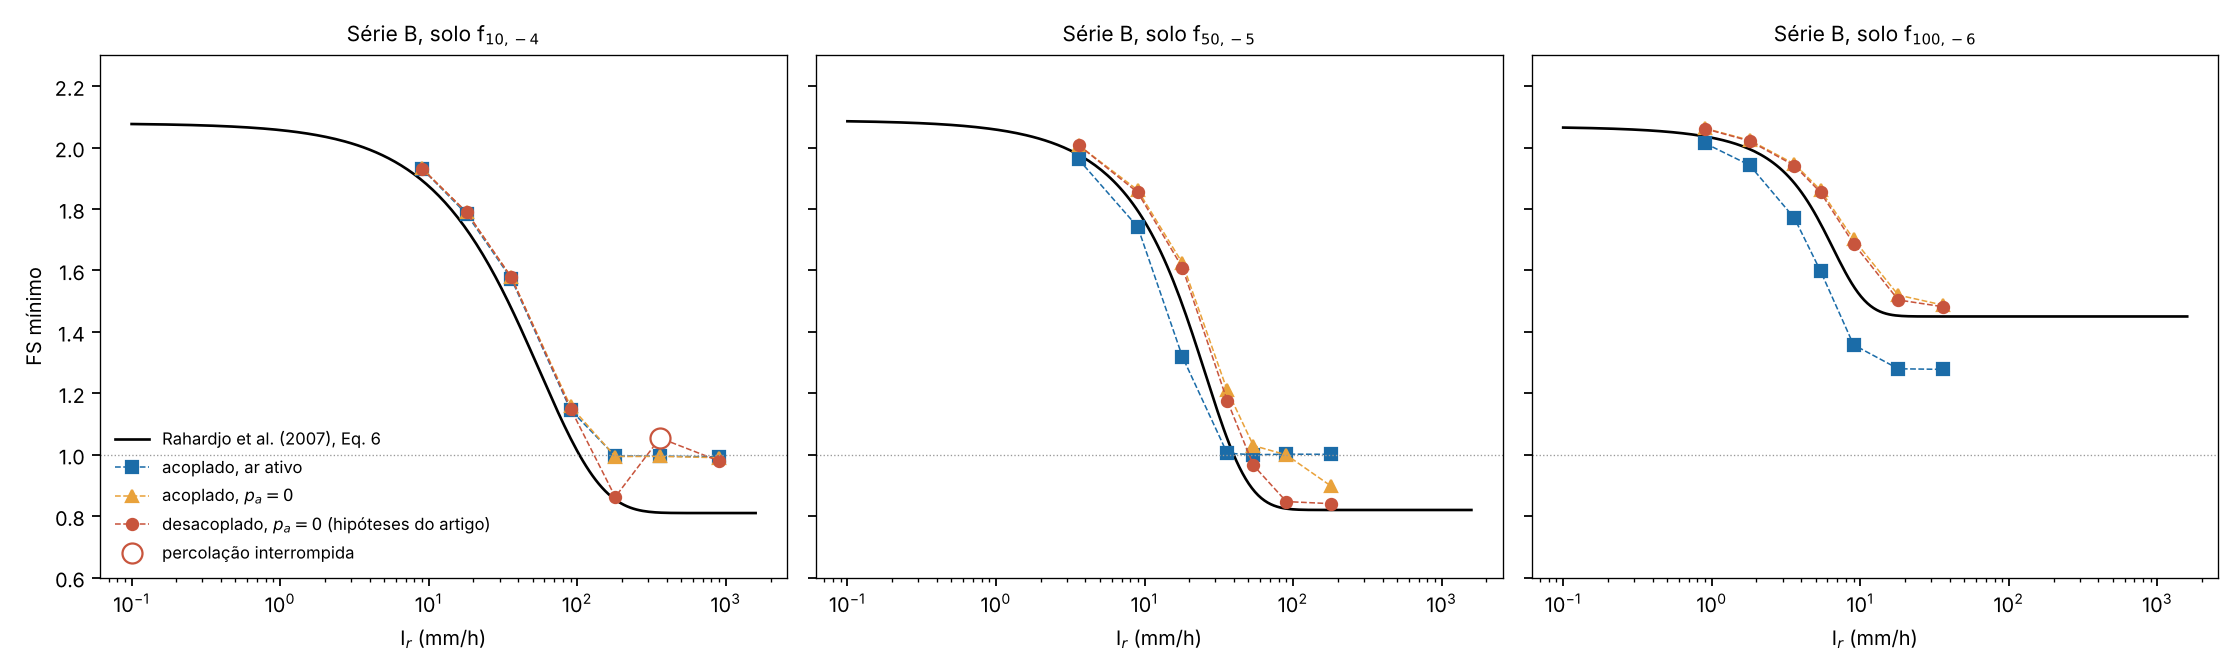
\includegraphics[width=\textwidth]{figuras/B_variantes_fsmin.png}
\caption{S\'erie B ($H_s=10$~m, $\alpha=45^\circ$, $H_w=5$~m, 24~h de chuva): FS m\'inimo $\times$ $I_r$ nas tr\^es
variantes do modelo e Eq.~6 do artigo (ajuste aos seus resultados, Fig.~7). C\'irculo vazado: percola\c{c}\~ao
interrompida antes do fim da chuva (m\'inimo superestimado).}\label{fig:Bvar}
\end{figure}

\begin{table}[htbp]
\centering
\caption{S\'erie B: FS m\'inimo. Eq.~6: ajuste do artigo; (i) modelo completo; (ii) ar passivo; (iii) desacoplado
com ar passivo (hip\'oteses do artigo). $^*$Percola\c{c}\~ao interrompida \`as 8,5~h (superf\'icie toda alagada).}
\label{tab:B}
\begin{tabular}{llcccc}
\toprule
Solo & $I_r$ (mm/h) & Eq.~6 & (i) completo & (ii) ar passivo & (iii) desacoplado\\
\midrule
$f_{10,-4}$ & 9 & 1,89 & 1,93 & 1,93 & 1,93\\
 & 36 & 1,48 & 1,57 & 1,58 & 1,58\\
 & 90 & 1,05 & 1,15 & 1,16 & 1,15\\
 & 180 & 0,85 & 1,00 & 0,99 & \textbf{0,86}\\
 & 360 & 0,81 & 1,00 & 1,00 & 1,05$^*$\\
 & 900 & 0,81 & 0,99 & 0,99 & 0,98$^*$\\
\midrule
$f_{50,-5}$ & 3,6 & 1,98 & 1,96 & 2,01 & 2,01\\
 & 9 & 1,79 & 1,74 & 1,86 & 1,85\\
 & 18 & 1,49 & 1,32 & 1,62 & 1,61\\
 & 36 & 1,05 & 1,01 & 1,21 & 1,18\\
 & 54 & 0,89 & 1,00 & 1,03 & \textbf{0,97}\\
 & 90 & 0,82 & 1,00 & 1,00 & \textbf{0,85}\\
 & 180 & 0,82 & 1,00 & 0,90 & \textbf{0,84}\\
\midrule
$f_{100,-6}$ & 0,9 & 2,04 & 2,01 & 2,06 & 2,06\\
 & 3,6 & 1,88 & 1,77 & 1,95 & 1,94\\
 & 9 & 1,55 & 1,36 & 1,70 & 1,69\\
 & 18 & 1,45 & 1,28 & 1,52 & 1,50\\
 & 36 & 1,45 & 1,28 & 1,49 & 1,48\\
\bottomrule
\end{tabular}
\end{table}

\begin{table}[htbp]
\centering
\caption{Solo $f_{50,-5}$: FS ao longo do tempo, Fig.~5b do artigo (digitalizada, $\pm0{,}03$) e NeoPZ
(modelo completo / desacoplado com ar passivo).}\label{tab:fig5b}
\begin{tabular}{lcccc}
\toprule
$I_r$ (mm/h) & $t=6$~h & $t=12$~h & $t=24$~h & $t=48$~h\\
\midrule
9 & 2,00 / 2,00 / 2,03 & 1,92 / 1,90 / 1,96 & 1,78 / 1,74 / 1,85 & 1,85 / 1,87 / 1,91\\
18 & 1,92 / 1,88 / 1,96 & 1,76 / 1,67 / 1,83 & 1,50 / 1,32 / 1,61 & 1,60 / 1,65 / 1,68\\
36 & 1,72 / 1,61 / 1,82 & 1,40 / 1,18 / 1,56 & 1,04 / 1,00 / 1,18 & 1,24 / 1,51 / 1,33\\
54 & 1,49 / 1,36 / 1,67 & 1,20 / 1,08 / 1,32 & 0,90 / 1,00 / 0,97 & 1,15 / 1,51 / 1,19\\
90 & 1,35 / 1,24 / 1,44 & 1,18 / 1,06 / 1,19 & 0,86 / 1,00 / 0,85 & 1,15 / 1,51 / 1,17\\
180 & 1,33 / 1,20 / 1,37 & 1,14 / 1,06 / 1,16 & 0,82 / 1,00 / 0,84 & 1,15 / 1,52 / 1,17\\
\bottomrule
\end{tabular}
\end{table}

\begin{figure}[htbp]
\centering
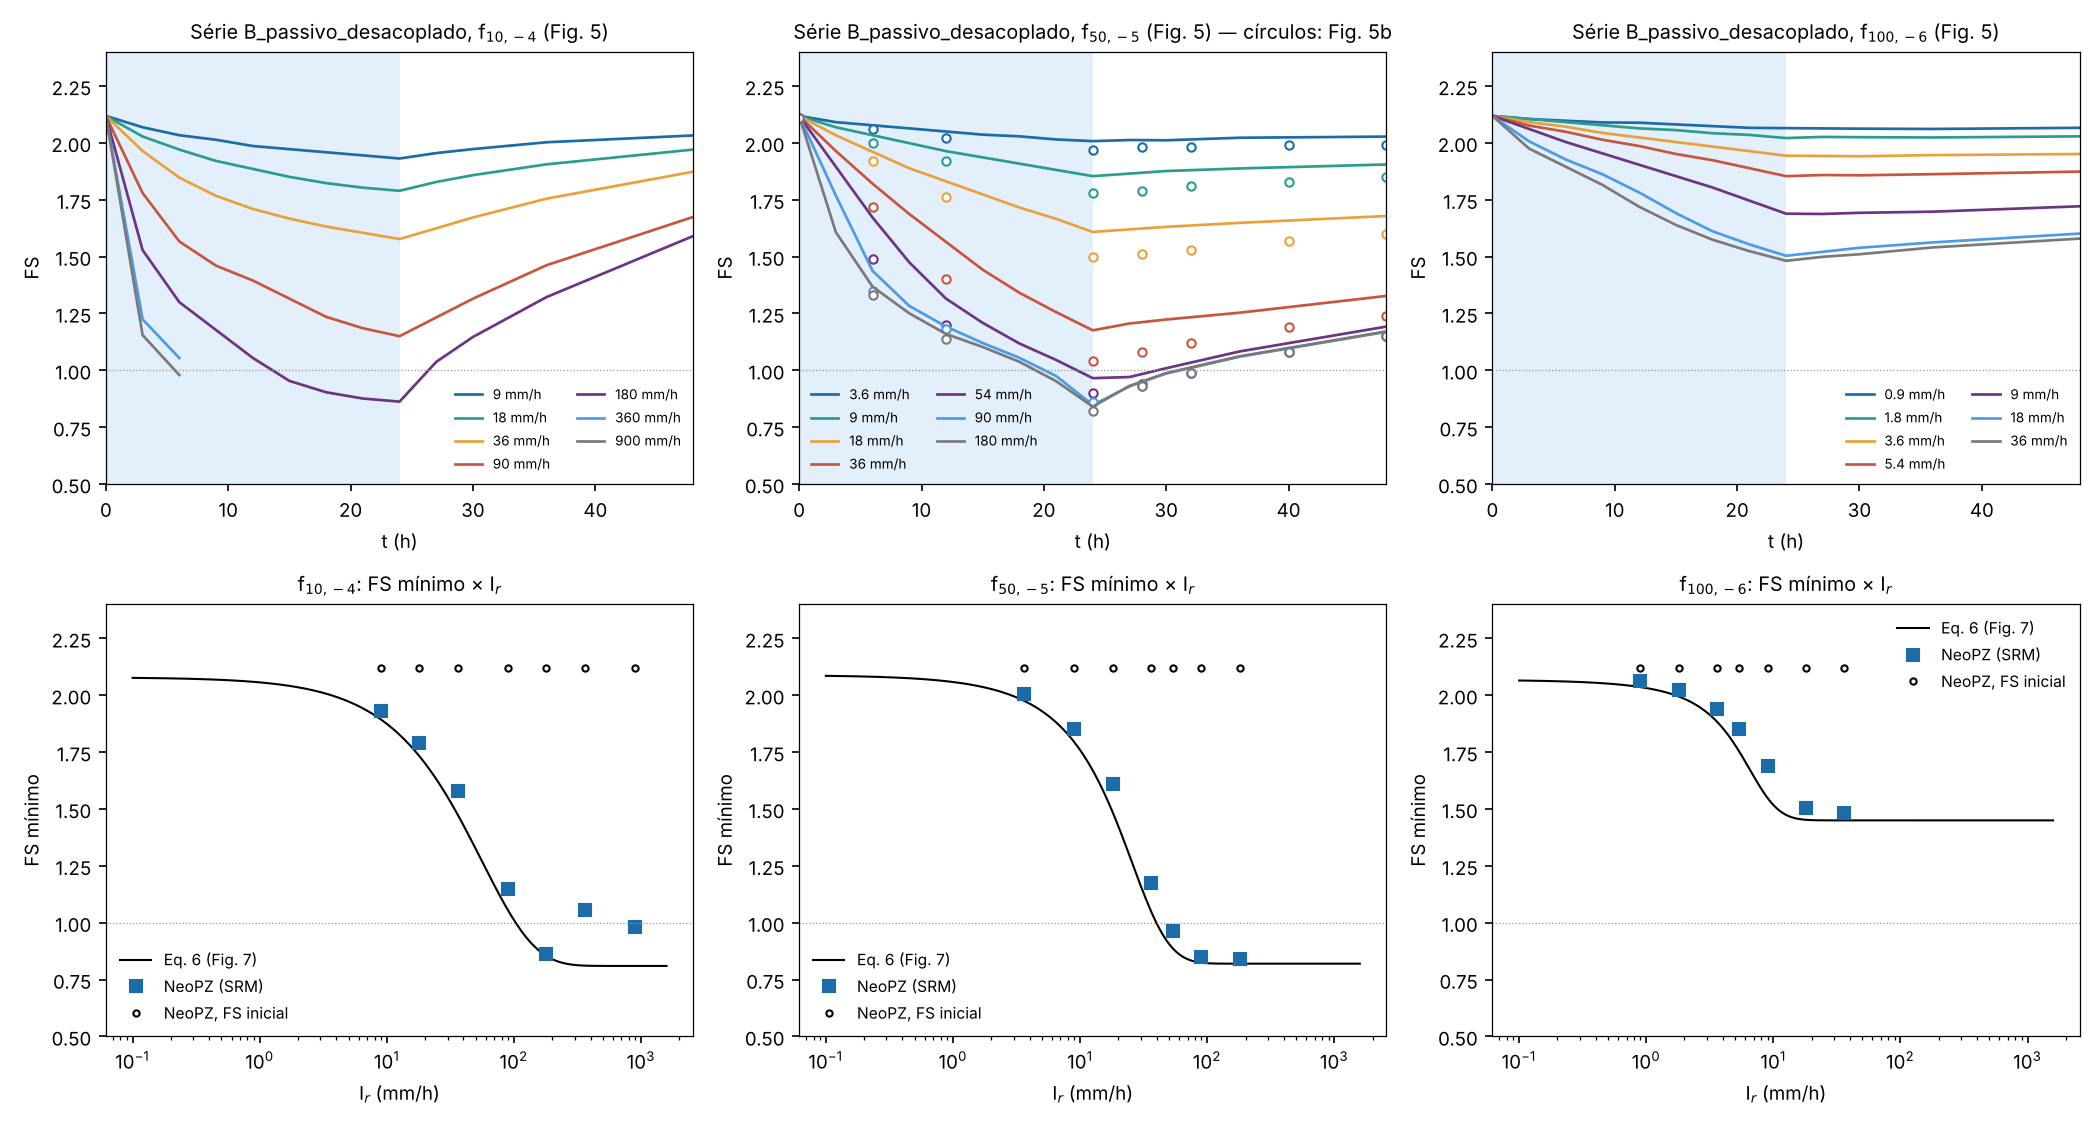
\includegraphics[width=\textwidth]{figuras/B_passivo_desacoplado_fs.png}
\caption{S\'erie B, desacoplado com ar passivo (hip\'oteses do artigo). Acima: FS($t$) (c\'irculos: Fig.~5b); abaixo:
FS m\'inimo $\times$ $I_r$ e Eq.~6.}\label{fig:Bdesac}
\end{figure}

\begin{figure}[htbp]
\centering
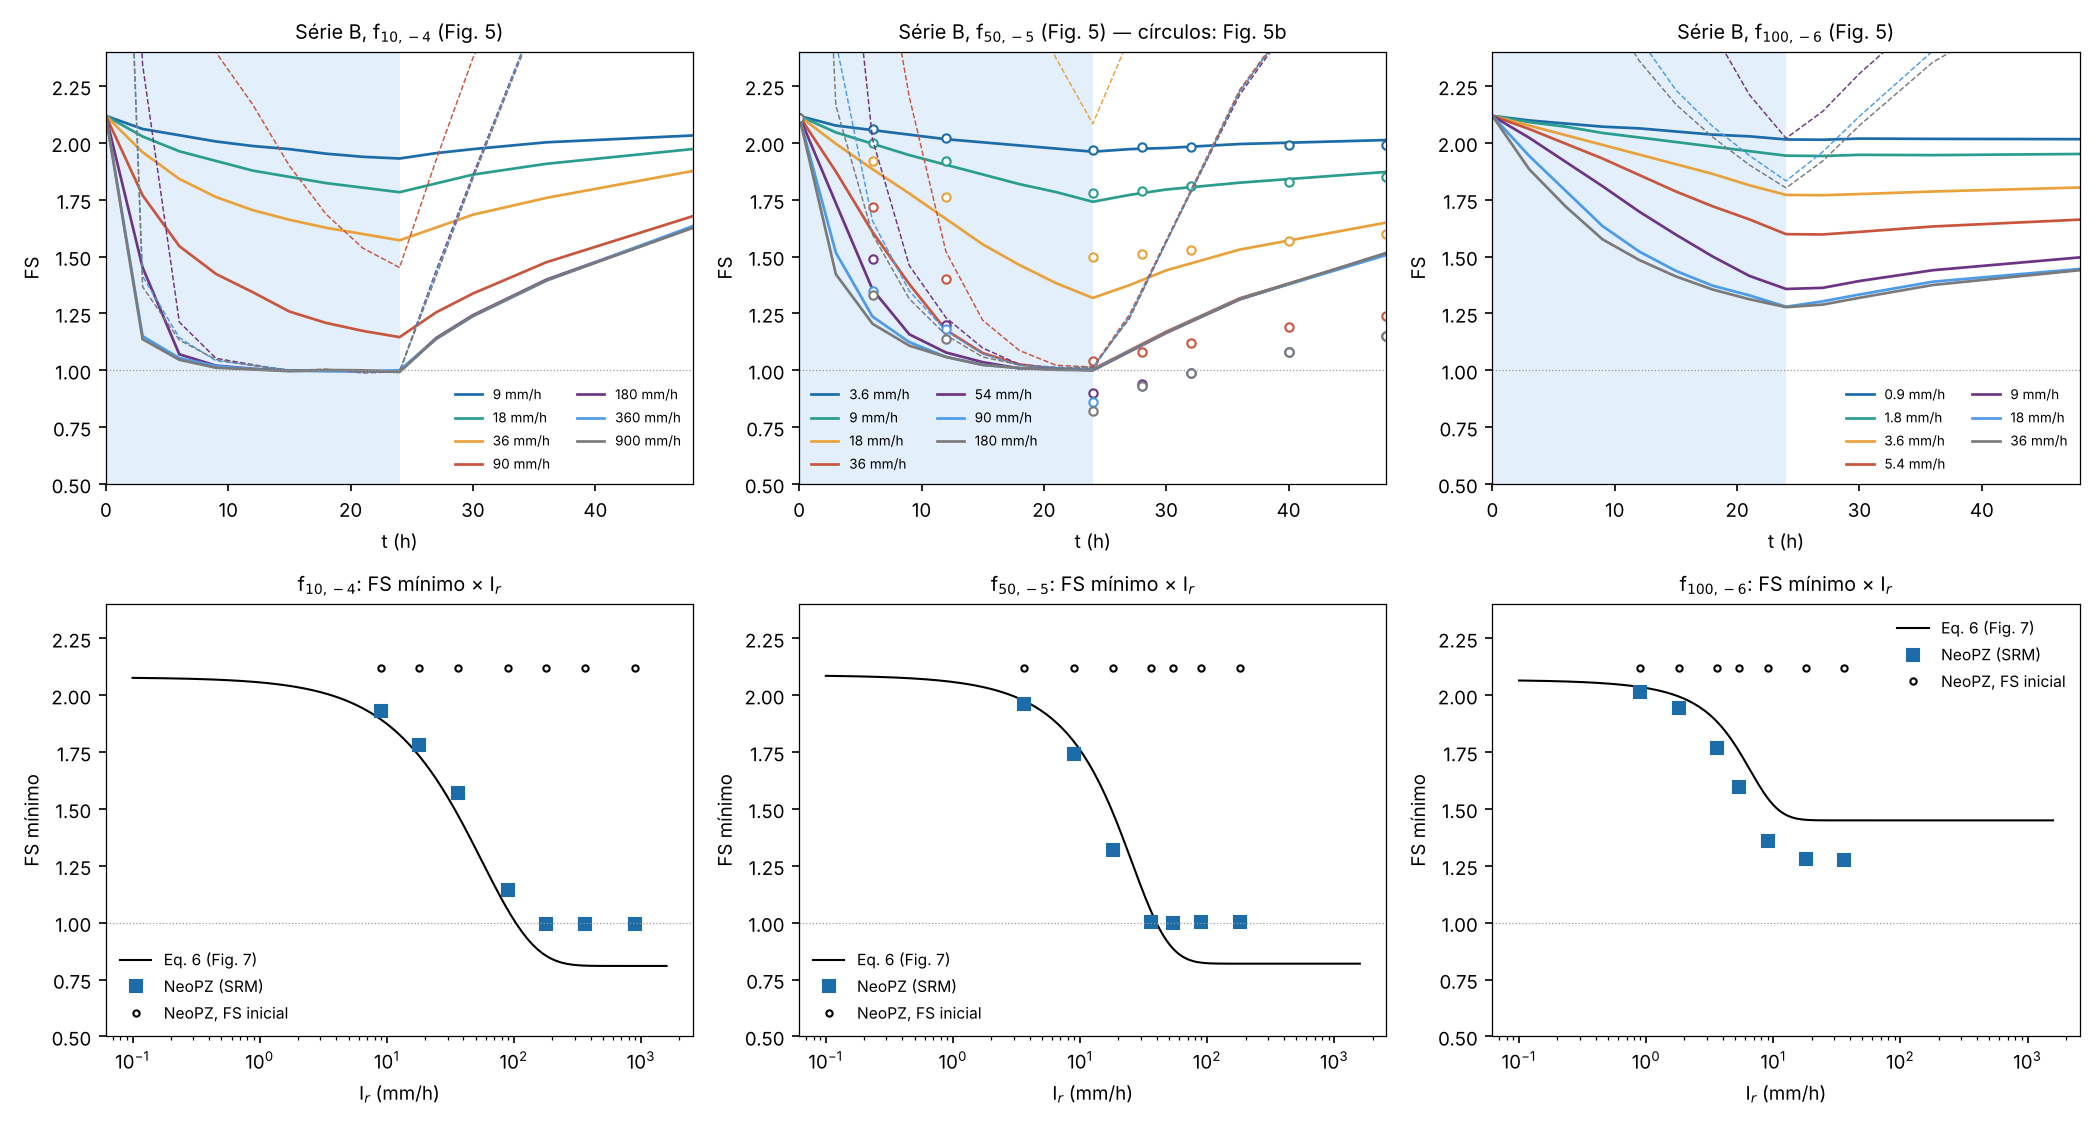
\includegraphics[width=\textwidth]{figuras/B_fs.png}
\caption{S\'erie B, modelo completo (acoplado, ar ativo). Linhas tracejadas: FS por aumento da gravidade.}
\label{fig:Bcomp}
\end{figure}

Observa\c{c}\~oes:
\begin{enumerate}
\item \textbf{Com as hip\'oteses do artigo} (variante iii) o FS m\'inimo segue a sigmoide da Eq.~6 nos tr\^es solos,
inclusive o patamar inferior (0,84--0,86 contra 0,81--0,82) e a recupera\c{c}\~ao depois da chuva da Fig.~5b. As
diferen\c{c}as restantes (FS 0,05--0,15 maior nas chuvas moderadas) s\~ao compat\'iveis com SRM $\times$ Bishop e com a
digitaliza\c{c}\~ao.
\item \textbf{No modelo completo o FS n\~ao desce abaixo de $\approx1{,}00$.} O transiente acoplado nunca perde o
equil\'ibrio: com Mohr--Coulomb associativo a plastifica\c{c}\~ao dilata o solo e, com o acoplamento
$S_w\alpha\,\dot\varepsilon_v$, a dilata\c{c}\~ao reduz $p_w$ (gera suc\c{c}\~ao) e aumenta a resist\^encia: o talude
estabiliza no limite. O mesmo patamar aparece nas S\'eries A, C e D. A recupera\c{c}\~ao depois da chuva \'e mais r\'apida
(FS 1,51 em 48~h contra 1,24).
\item \textbf{O ar ativo reduz o FS nos solos pouco perme\'aveis} ($f_{100}$ com 18~mm/h: 1,28 contra 1,50 com
$p_a=0$; $f_{50}$ com 18~mm/h: 1,32 contra 1,62). O ar aprisionado sob a frente de umedecimento chega a 50~kPa
(Fig.~\ref{fig:campos}) e eleva $p_w$ (positiva sob a crista, com suc\c{c}\~ao ainda positiva); com $\chi=1$ a
tens\~ao efetiva depende de $p_w$.
\item O FS por aumento da gravidade \'e muito maior que o SRM no estado inicial (5,7 contra 2,1), porque a suc\c{c}\~ao
mantida \'e uma parcela de resist\^encia que n\~ao cresce com o peso; os dois coincidem perto da ruptura
(Fig.~\ref{fig:fstempo}).
\end{enumerate}

\begin{figure}[htbp]
\centering
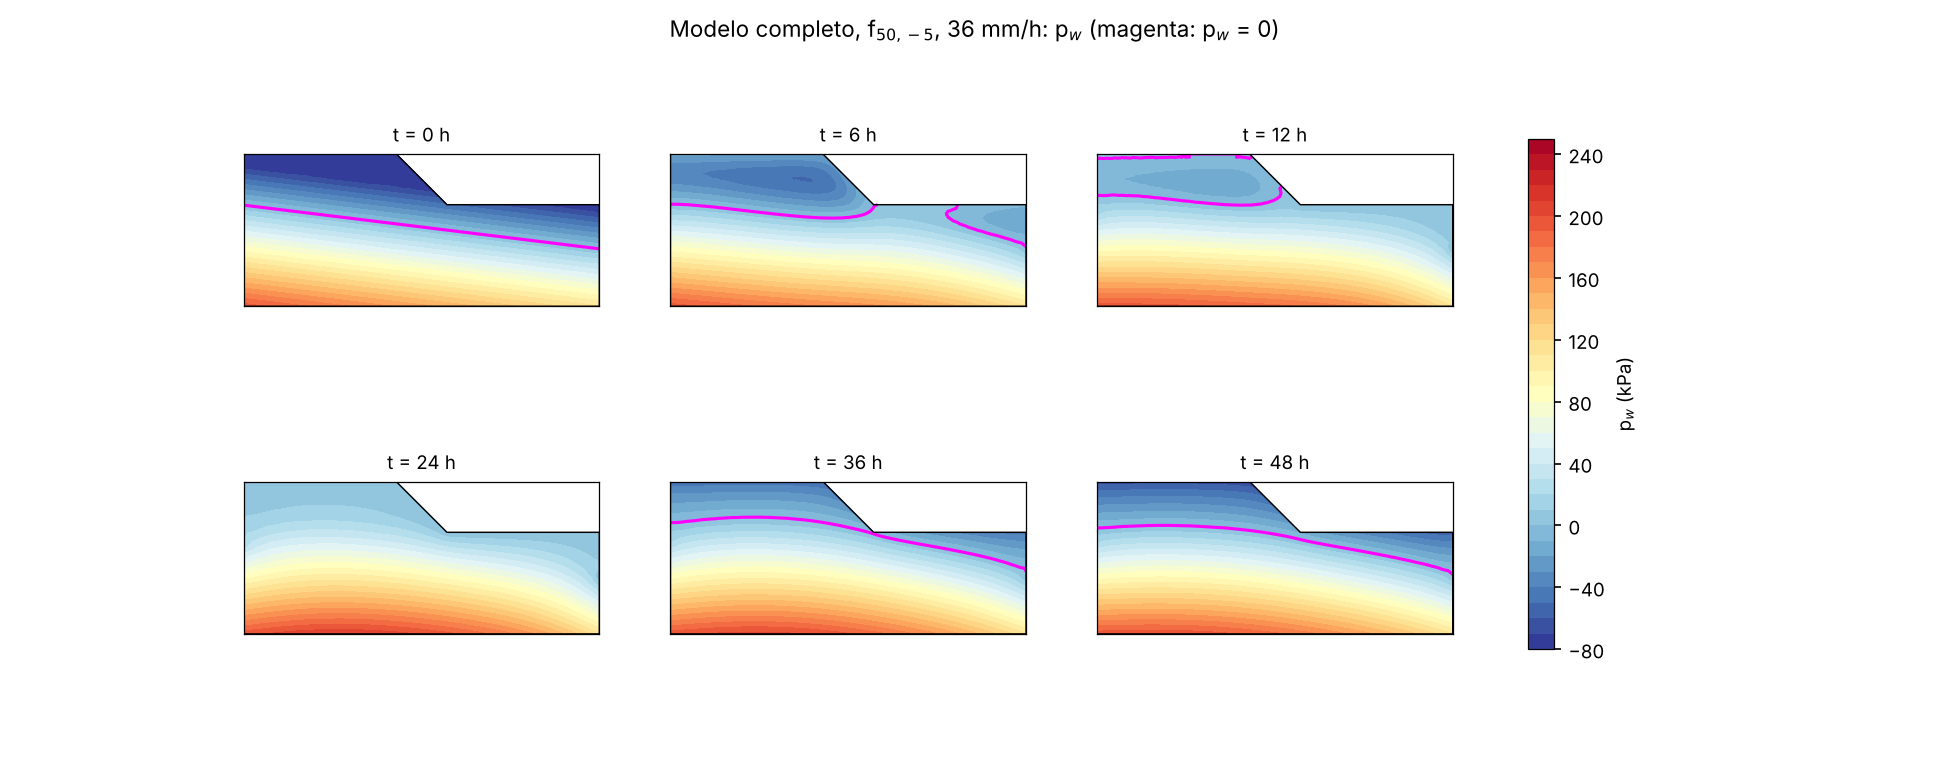
\includegraphics[width=0.95\textwidth]{figuras/campos_pw_f50_a45_H10_Hw5_I36_B.png}\\
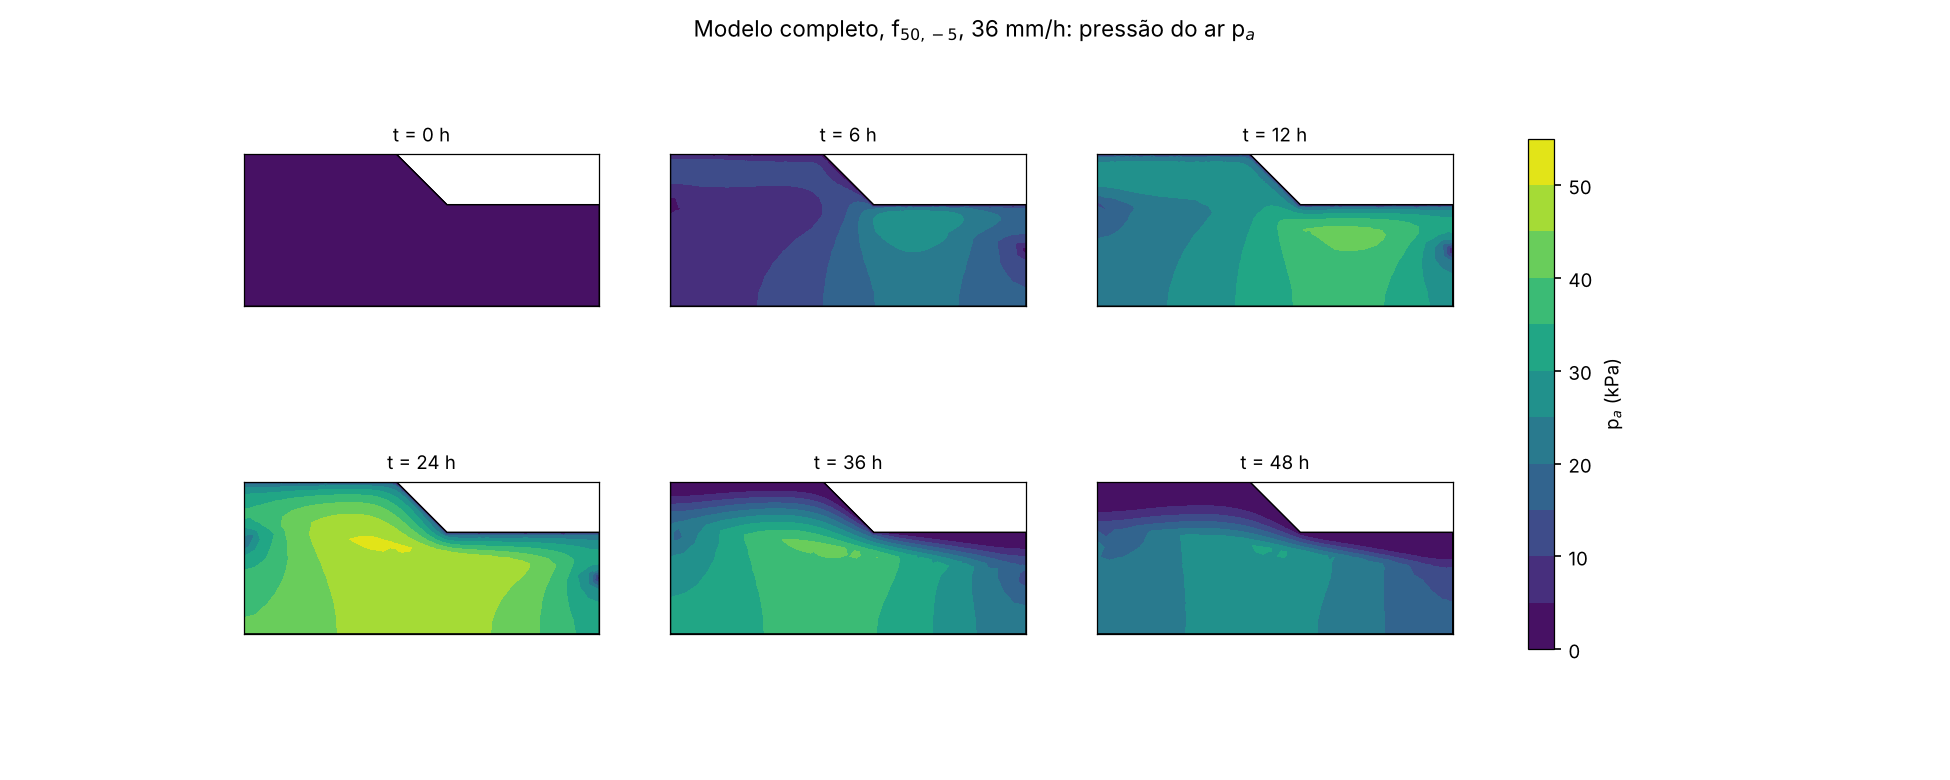
\includegraphics[width=0.95\textwidth]{figuras/campos_pa_f50_a45_H10_Hw5_I36_B.png}\\
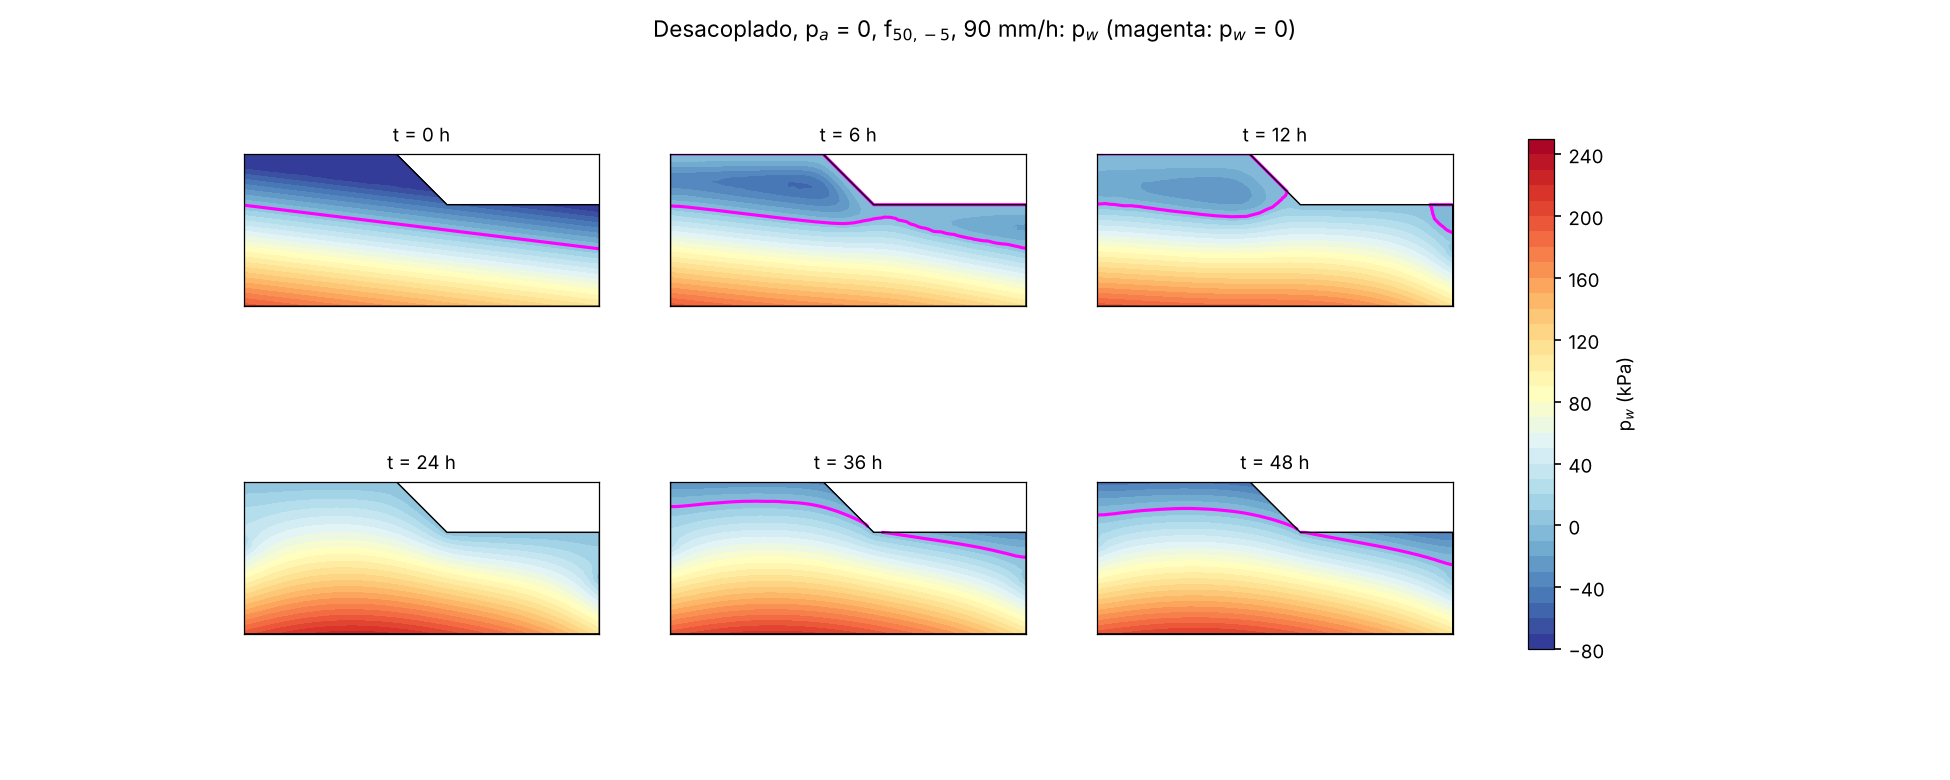
\includegraphics[width=0.95\textwidth]{figuras/campos_pw_f50_a45_H10_Hw5_I90_B_passivo_desacoplado.png}
\caption{Campos de press\~ao. Acima e no meio: modelo completo, $f_{50,-5}$, 36~mm/h ($p_w$ e $p_a$); o ar
pressurizado sob a frente de umedecimento torna $p_w$ positiva perto da superf\'icie. Abaixo: desacoplado com ar
passivo, 90~mm/h: eleva\c{c}\~ao do len\c{c}ol fre\'atico at\'e a face (categoria I/II da Tabela~3 do artigo).}
\label{fig:campos}
\end{figure}

\subsection{S\'erie A: \^angulo do talude}

A Tabela~7 do artigo n\~ao reproduz a pr\'opria Fig.~9 em algumas linhas (por exemplo, $f_{10}$ com 80~mm/h:
$2{,}830-0{,}027\cdot26{,}6=2{,}11$ na tabela e $\approx1{,}45$ na figura). A compara\c{c}\~ao usa os pontos lidos da
Fig.~9 ($\pm0{,}05$), Tabela~\ref{tab:A} e Fig.~\ref{fig:A}.

\begin{table}[htbp]
\centering
\caption{S\'erie A: FS m\'inimo, NeoPZ (modelo completo) / Fig.~9, para $\alpha=26{,}6$; 33,7; 45 e $63{,}4^\circ$.}
\label{tab:A}
\begin{tabular}{llcccc}
\toprule
Solo & $I_r$ (mm/h) & $26{,}6^\circ$ & $33{,}7^\circ$ & $45^\circ$ & $63{,}4^\circ$\\
\midrule
$f_{10,-4}$ & 9 & 2,37 / 2,35 & 2,17 / 2,16 & 1,93 / 1,88 & 1,60 / 1,45\\
 & 80 & 1,51 / 1,45 & 1,37 / 1,32 & 1,19 / 1,12 & 1,00 / 0,83\\
 & 360 & 1,21 / 1,15 & 1,07 / 1,00 & 0,99 / 0,82 & 0,99 / 0,62\\
$f_{50,-5}$ & 9 & 2,14 / 2,27 & 1,96 / 2,07 & 1,74 / 1,79 & 1,46 / 1,36\\
 & 36 & 1,34 / 1,43 & 1,16 / 1,27 & 1,01 / 1,04 & 0,74 / 0,76\\
 & 80 & 1,33 / 1,15 & 1,15 / 1,00 & 1,00 / 0,82 & 1,00 / 0,67\\
$f_{100,-6}$ & 3,6 & 2,18 / 2,37 & 1,99 / 2,19 & 1,77 / 1,89 & 1,49 / 1,45\\
 & 9 & 1,84 / 2,12 & 1,61 / 1,92 & 1,36 / 1,55 & 1,17 / 1,11\\
 & 80 & 1,77 / 2,05 & 1,53 / 1,83 & 1,27 / 1,45 & 1,01 / 1,05\\
\bottomrule
\end{tabular}
\end{table}

\begin{figure}[htbp]
\centering
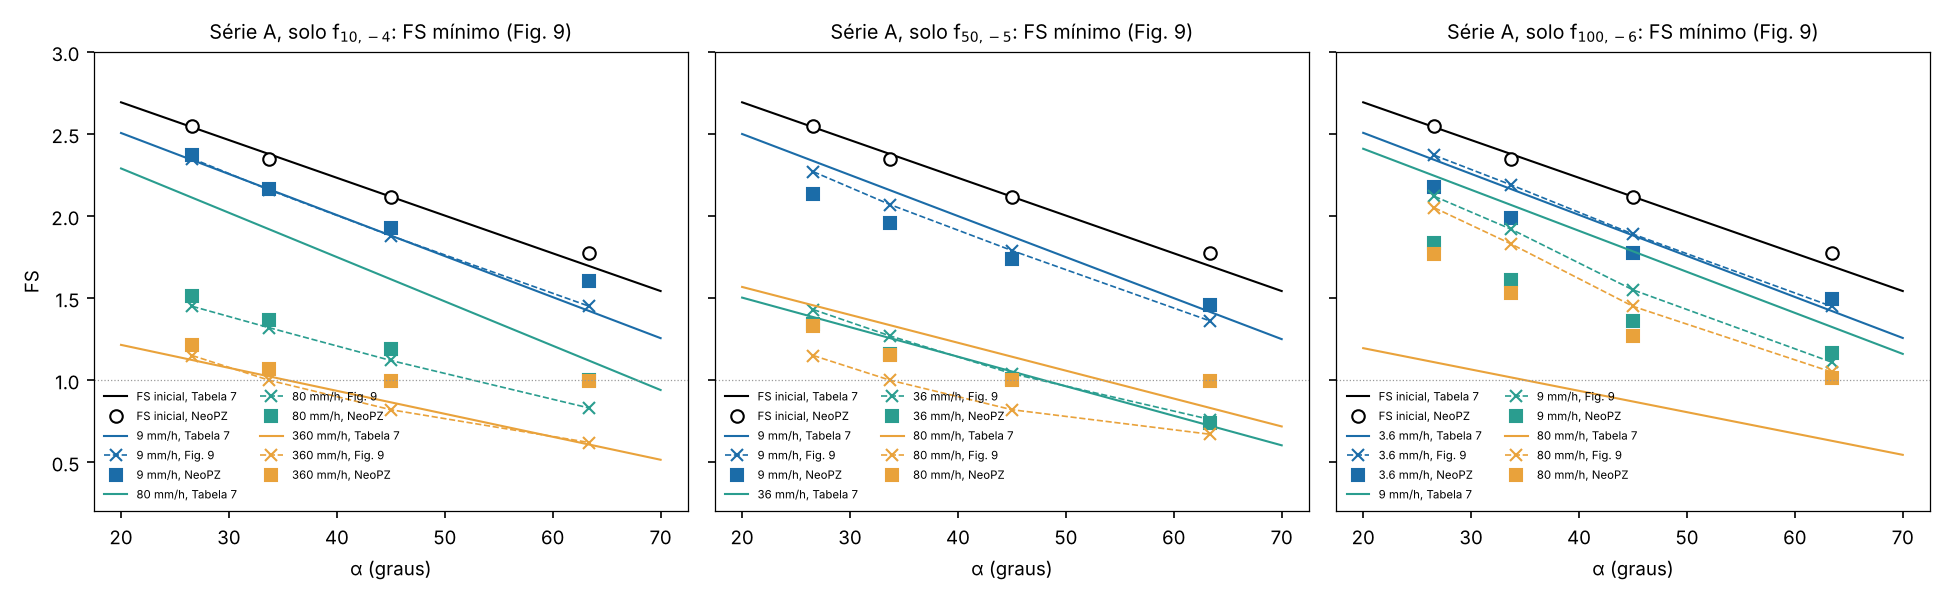
\includegraphics[width=\textwidth]{figuras/A_fs_min_alpha.png}
\caption{S\'erie A: FS inicial e m\'inimo $\times$ $\alpha$; linhas: Tabela~7; $\times$: Fig.~9; quadrados: NeoPZ.}
\label{fig:A}
\end{figure}

\begin{figure}[htbp]
\centering
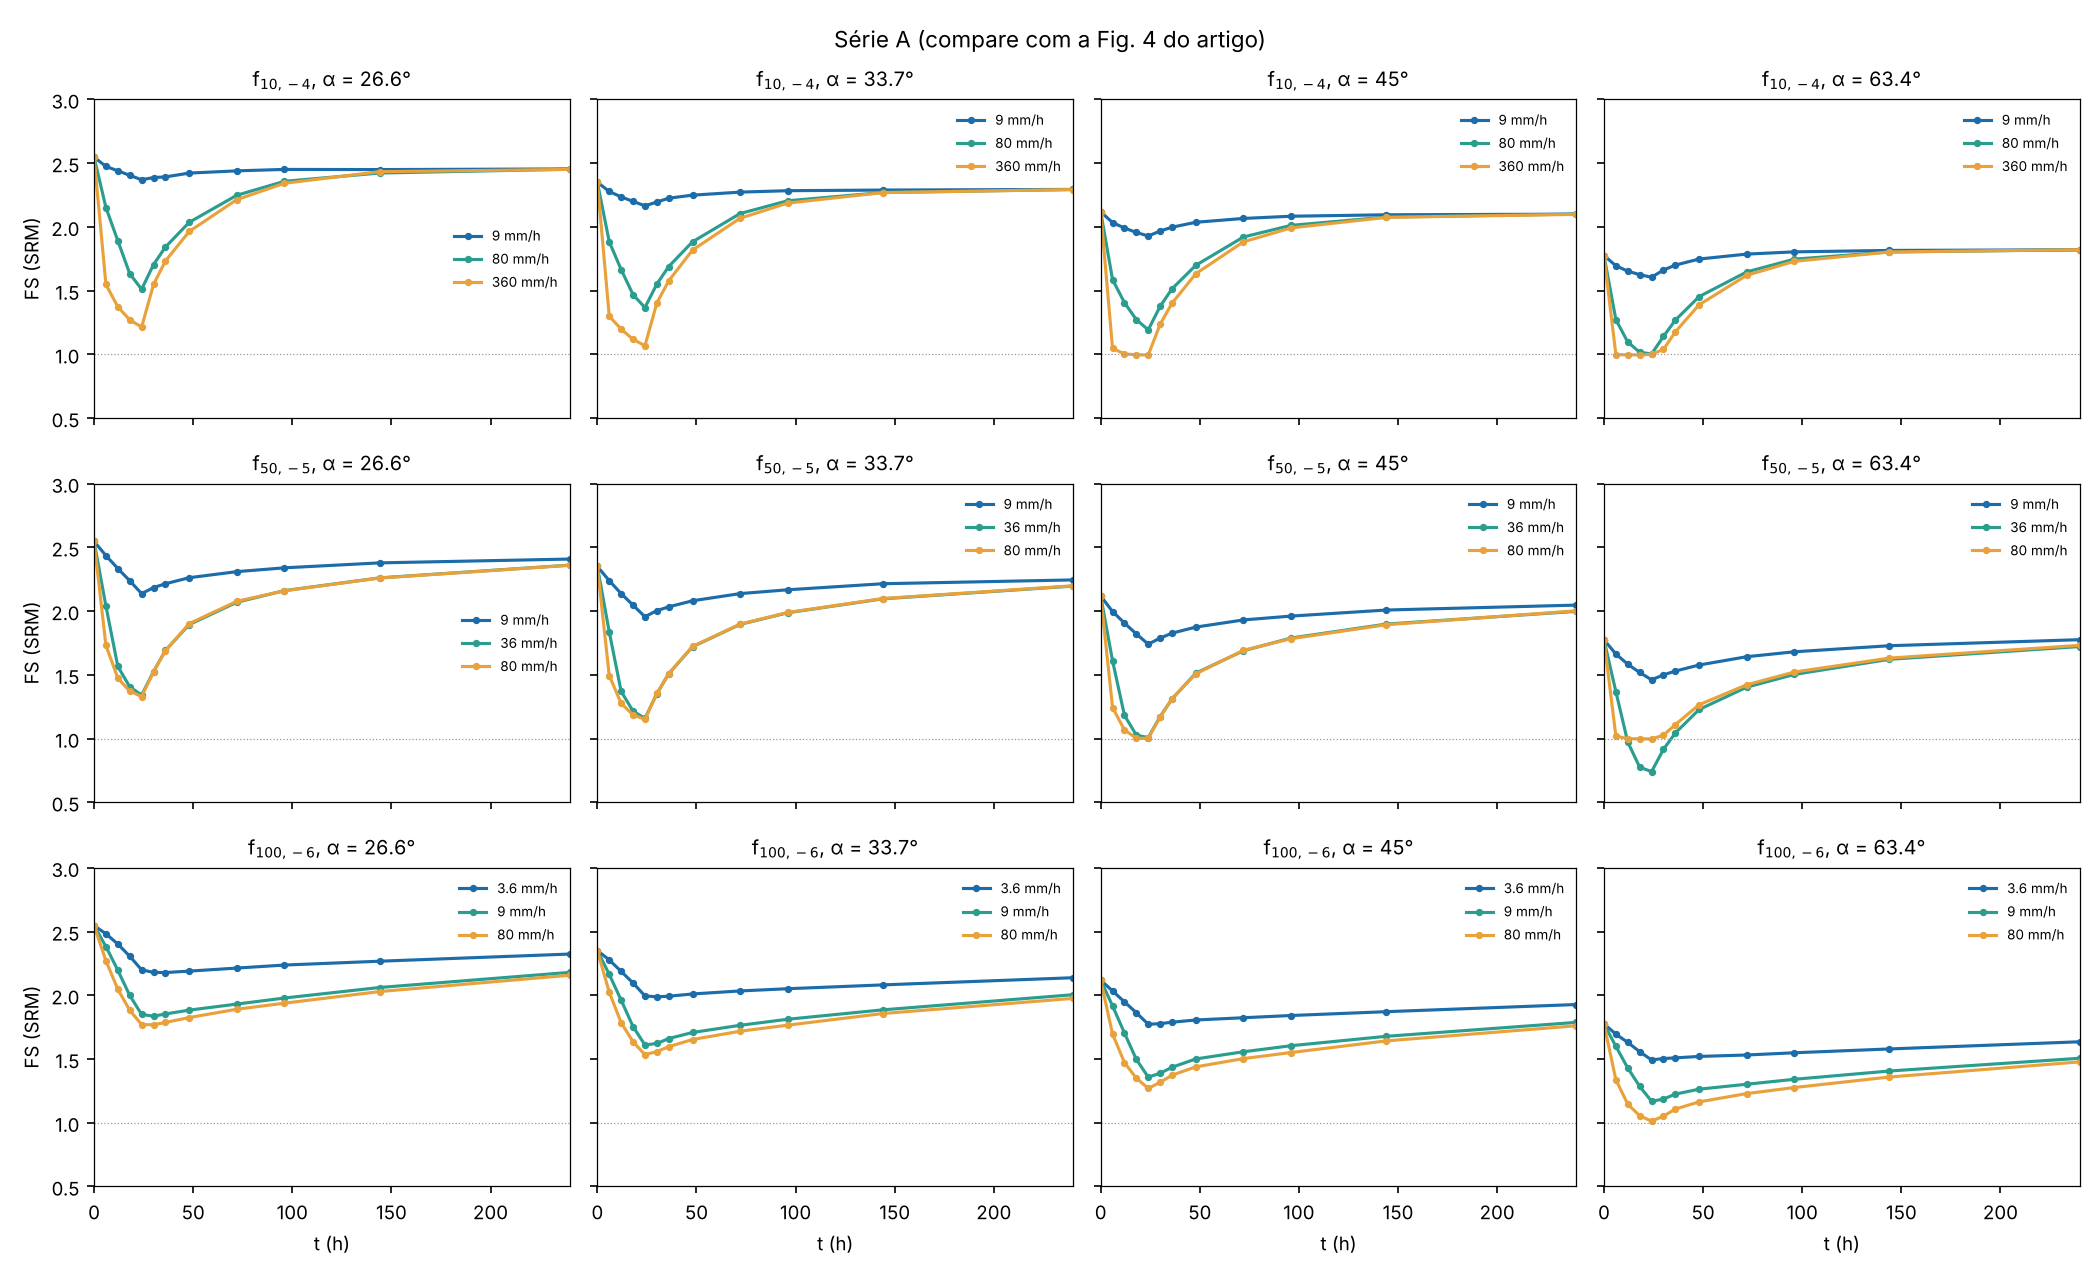
\includegraphics[width=\textwidth]{figuras/A_fs_tempo.png}
\caption{S\'erie A: FS($t$) at\'e 240~h (compare com a Fig.~4 do artigo).}\label{fig:A4}
\end{figure}

Nas chuvas fracas e moderadas o FS m\'inimo fica sobre a Fig.~9 (diferen\c{c}as at\'e 0,1, maiores no $f_{100}$, onde o
ar ativo reduz o FS); nas chuvas fortes aparece o patamar $\approx1$ do modelo acoplado. A diminui\c{c}\~ao do FS com
$\alpha$ \'e reproduzida: com 36~mm/h no $f_{50}$ o talude a $63{,}4^\circ$ rompe (0,74 contra 0,76; o transiente
perde o equil\'ibrio em $t=8$~h).

\subsection{S\'eries C e D: len\c{c}ol fre\'atico e altura}

\begin{table}[htbp]
\centering
\caption{S\'eries C e D: FS m\'inimo, NeoPZ (modelo completo) / Figs.~8 e 10.}\label{tab:CD}
\begin{tabular}{lccccc}
\toprule
S\'erie C, $H_w$ & 2,5~m & 5~m & 7,5~m & 10~m & 15~m\\
\midrule
9 mm/h & 1,38 / 1,43 & 1,74 / 1,79 & 2,01 / 2,00 & 2,17 / 2,13 & 2,31 / 2,20\\
36 mm/h & 1,00 / 0,85 & 1,00 / 1,04 & 1,03 / 1,19 & 1,08 / 1,26 & 1,14 / 1,29\\
80 mm/h & 1,00 / 0,81 & 1,00 / 0,82 & 1,01 / 1,05 & 1,04 / 1,15 & 1,09 / 1,16\\
\midrule
S\'erie D, $H_s$ & 5~m & 10~m & 20~m & 40~m & \\
\midrule
9 mm/h & 2,38 / 2,48 & 1,74 / 1,79 & 1,32 / 1,37 & 1,07 / 1,08 & \\
36 mm/h & 1,33 / 1,20 & 1,00 / 1,04 & 0,86 / 0,97 & 1,00 / 0,90 & \\
80 mm/h & 1,33 / 1,19 & 1,00 / 0,82 & 0,99 / 0,88 & 0,99 / 0,83 & \\
\bottomrule
\end{tabular}
\end{table}

\begin{figure}[htbp]
\centering
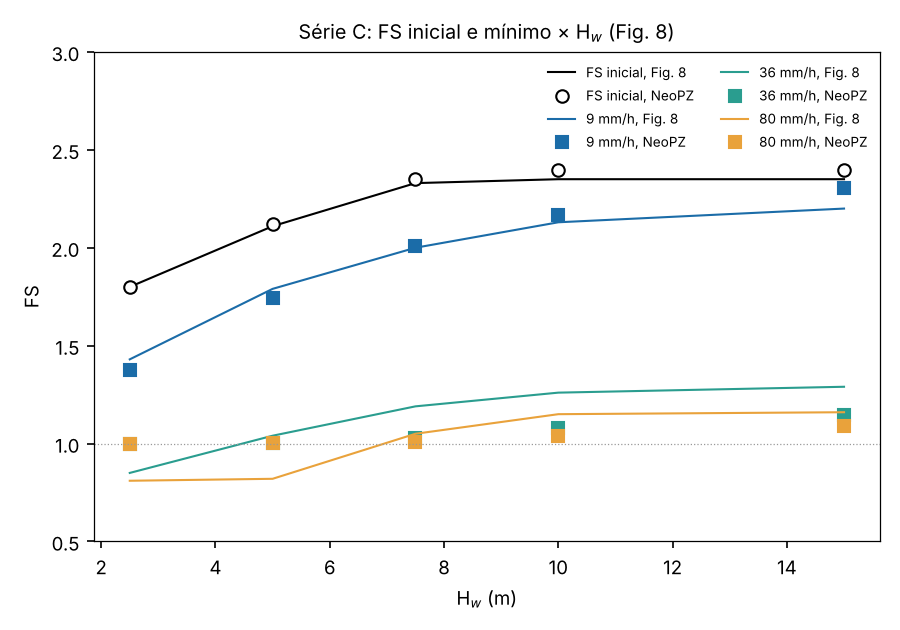
\includegraphics[width=0.49\textwidth]{figuras/C_fs_hw.png}\hfill
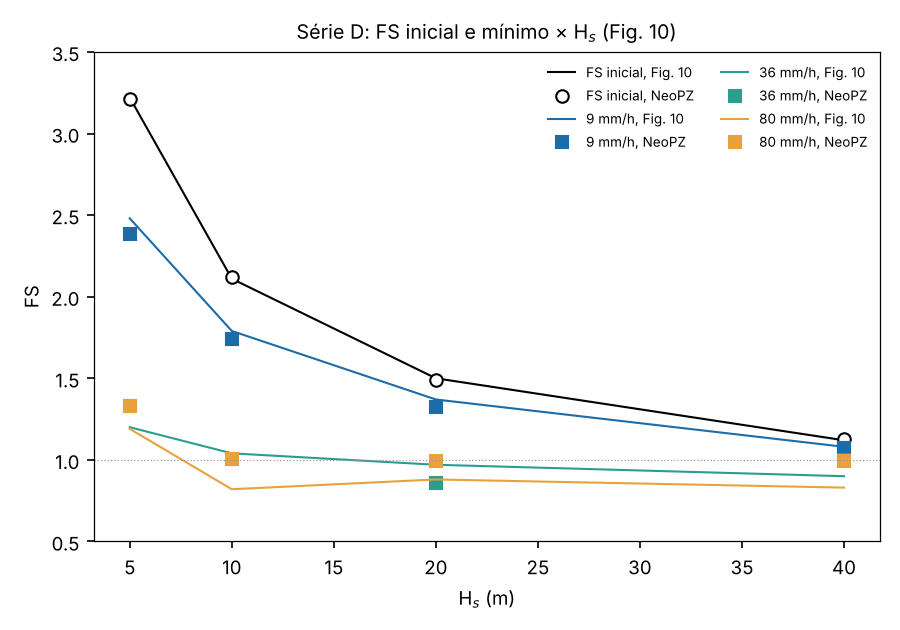
\includegraphics[width=0.49\textwidth]{figuras/D_fs_hs.png}
\caption{S\'eries C (esquerda, Fig.~8) e D (direita, Fig.~10): FS inicial e m\'inimo.}\label{fig:CD}
\end{figure}

Com 9~mm/h as S\'eries C e D reproduzem as Figs.~8 e 10 (diferen\c{c}as $\le0{,}11$). Nas chuvas de 36 e 80~mm/h o
FS do modelo acoplado volta ao patamar $\approx1$; os casos com $H_s=5$~m ficam acima do artigo (1,33 contra 1,20)
e o de 20~m com 36~mm/h abaixo (0,86 contra 0,97).

\subsection{Anisotropia da permeabilidade}

Solo $f_{50,-5}$, $\alpha=45^\circ$, $H_s=10$~m, $H_w=5$~m, 36~mm/h ($=k_s$) durante 24~h, modelo completo; o caso
isotr\'opico tem FS m\'inimo 1,005 (Tabelas~\ref{tab:aniso} e \ref{tab:rot}, Figs.~\ref{fig:aniso} e \ref{fig:rot}).

\begin{table}[htbp]
\centering
\caption{Tensor diagonal: FS m\'inimo e volume infiltrado em 24~h.}\label{tab:aniso}
\begin{tabular}{cccccc}
\toprule
$k_x$ (m/s) & $k_y$ (m/s) & $k_x/k_y$ & FS m\'in SRM & FS m\'in GI & infiltra\c{c}\~ao (m$^3$/m)\\
\midrule
$10^{-5}$ & $10^{-5}$ & 1 & 1,005 & 1,01 & 38,4\\
$3\cdot10^{-5}$ & $10^{-5}$ & 3 & 1,035 & 1,10 & 40,2\\
$10^{-4}$ & $10^{-5}$ & 10 & 1,078 & 1,25 & 42,7\\
$10^{-5}$ & $10^{-6}$ & 10 & 1,259 & 1,75 & 16,0\\
$10^{-6}$ & $10^{-5}$ & 0,1 & 1,002 & 1,01 & 35,5\\
$10^{-5}$ & $10^{-4}$ & 0,1 & 1,195 & 1,56 & 53,9\\
\bottomrule
\end{tabular}
\end{table}

\begin{table}[htbp]
\centering
\caption{Tensor girado: $k_1=10^{-4}$~m/s na dire\c{c}\~ao $\theta$, $k_2=10^{-5}$~m/s normal a ela. A face desce a
$-45^\circ$: $\theta=135^\circ$ \'e a dire\c{c}\~ao da face.}\label{tab:rot}
\setlength{\tabcolsep}{4pt}
\begin{tabular}{lcccccccccccc}
\toprule
$\theta$ ($^\circ$) & 0 & 15 & 30 & 45 & 60 & 75 & 90 & 105 & 120 & 135 & 150 & 165\\
\midrule
FS m\'in SRM & 1,08 & 1,19 & 1,33 & 1,33 & 1,28 & 1,24 & 1,20 & 1,16 & 1,15 & 1,18 & 1,20 & 1,11\\
FS m\'in GI & 1,24 & 1,64 & 2,21 & 2,16 & 1,95 & 1,73 & 1,55 & 1,42 & 1,37 & 1,49 & 1,60 & 1,36\\
Infiltra\c{c}\~ao (m$^3$/m) & 43,0 & 48,1 & 52,9 & 53,8 & 53,7 & 53,7 & 53,9 & 54,8 & 56,3 & 57,9 & 57,3 & 50,0\\
\bottomrule
\end{tabular}
\end{table}

\begin{figure}[htbp]
\centering
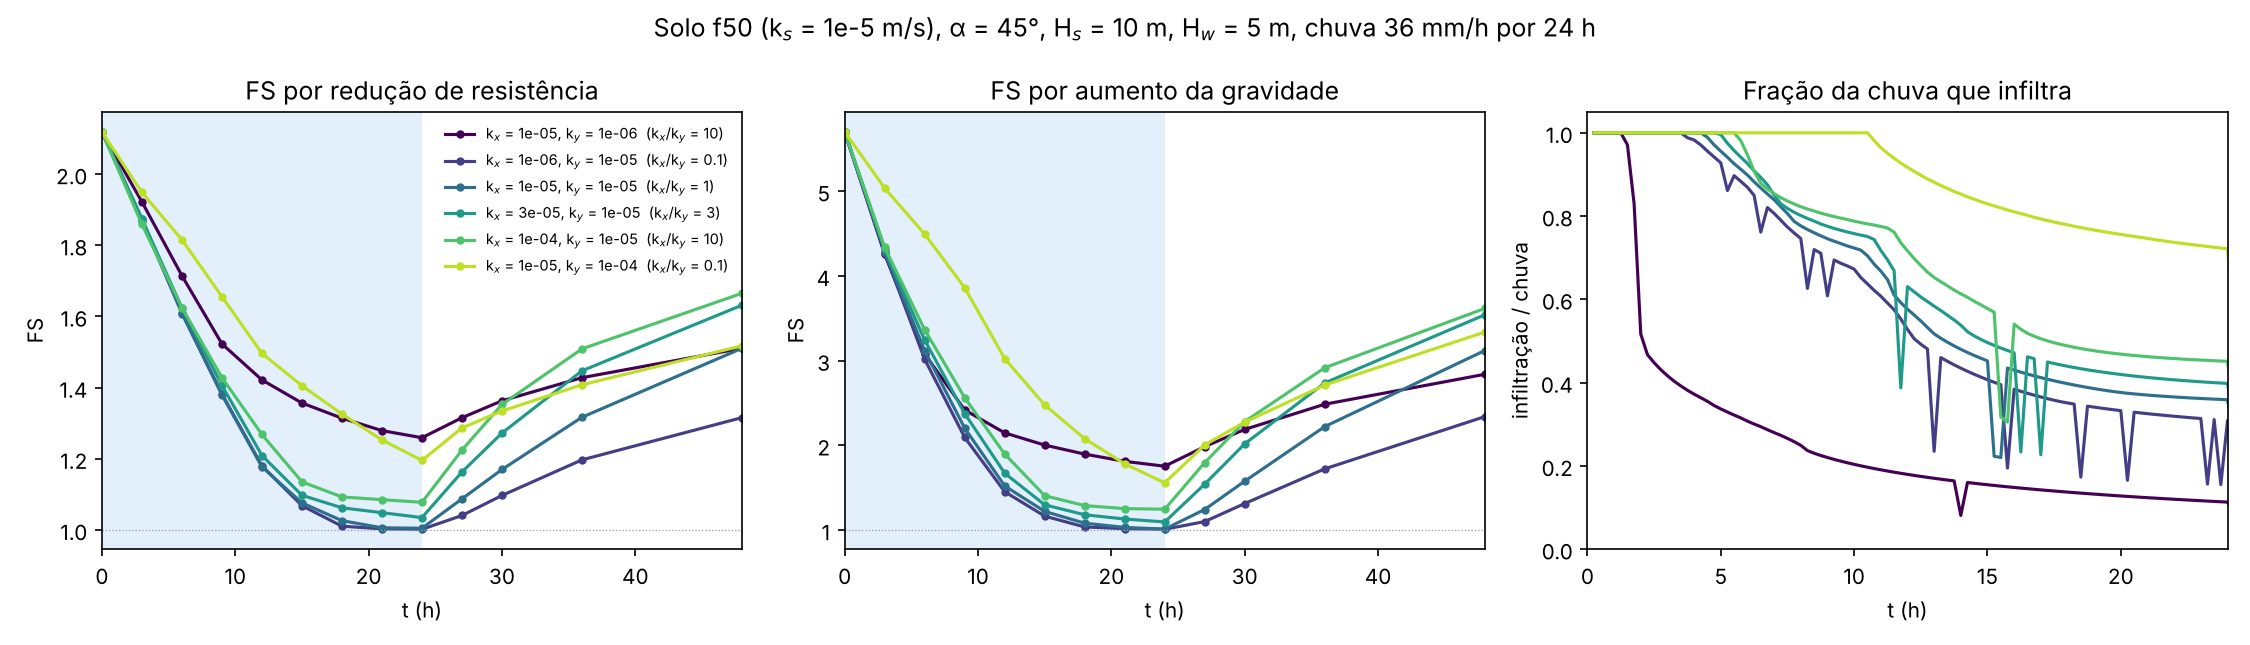
\includegraphics[width=\textwidth]{figuras/anisotropia_fs.png}
\caption{Tensor diagonal: FS($t$) por redu\c{c}\~ao de resist\^encia e por aumento da gravidade, e fra\c{c}\~ao da chuva
que infiltra.}\label{fig:aniso}
\end{figure}

\begin{figure}[htbp]
\centering
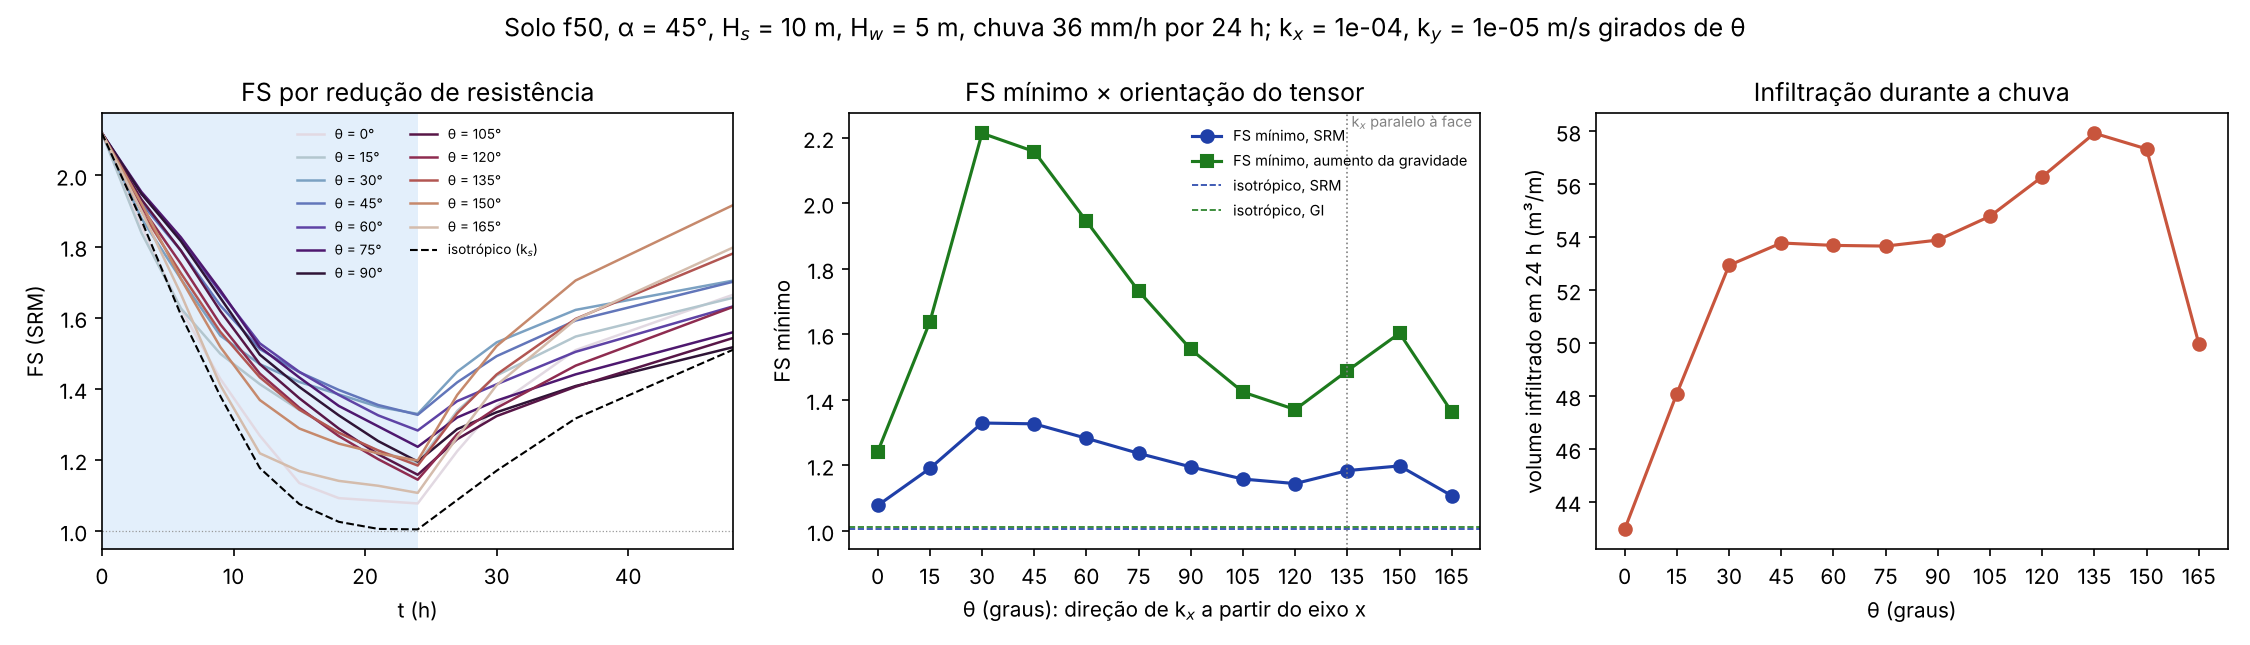
\includegraphics[width=\textwidth]{figuras/rotacao_fs.png}
\caption{Tensor girado de $15^\circ$ em $15^\circ$: FS($t$), FS m\'inimo $\times$ $\theta$ e infiltra\c{c}\~ao.}
\label{fig:rot}
\end{figure}

\begin{itemize}
\item Com $k_y<k_s$ a chuva infiltra menos (escoa na superf\'icie) e o FS sobe (1,26); com $k_x>k_y$ a \'agua se
espalha lateralmente e drena pela face.
\item Com $k_y>k_x$ infiltra mais \'agua (53,9 m$^3$/m), mas o FS tamb\'em sobe (1,20): a frente desce r\'apido e
drena, sem saturar a zona rasa.
\item Girando o tensor, o pior caso \'e $\theta=0$ (estratifica\c{c}\~ao horizontal) e o melhor $\theta\approx30$--$45^\circ$
(dire\c{c}\~ao mais perme\'avel subindo para dentro do maci\c{c}o, contr\'aria \`a face): a \'agua \'e conduzida para longe
da face. Todos os casos anisotr\'opicos ficam acima do isotr\'opico com o mesmo $k_{\min}=k_s$.
\end{itemize}

\subsection{P\'os-processamento}

Para cada caso, o script \texttt{animacao.py} (ou \texttt{mma/animacao.wl} no Mathematica) gera o FS em escala
$\log t$ (Fig.~\ref{fig:fstempo}; $t=0$ desenhado em 0,01~h, linha vertical no instante de ruptura do transiente) e
uma anima\c{c}\~ao das isolinhas de $p_w$ (preenchimento a cada 10~kPa, isolinhas rotuladas a cada 50~kPa, $p_w=0$
em magenta) ao lado do gr\'afico do FS, com o marcador do instante interpolado linearmente em $\log t$.

\begin{figure}[htbp]
\centering
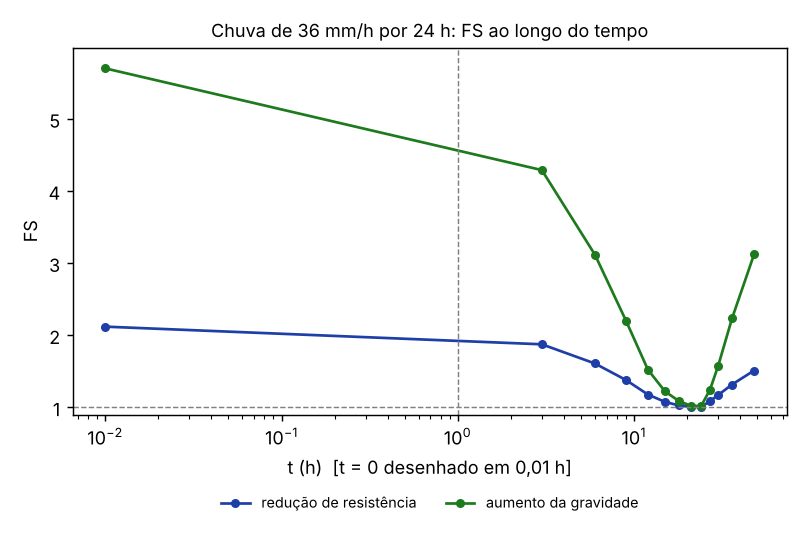
\includegraphics[width=0.48\textwidth]{figuras/fs_tempo_f50_I36.png}\hfill
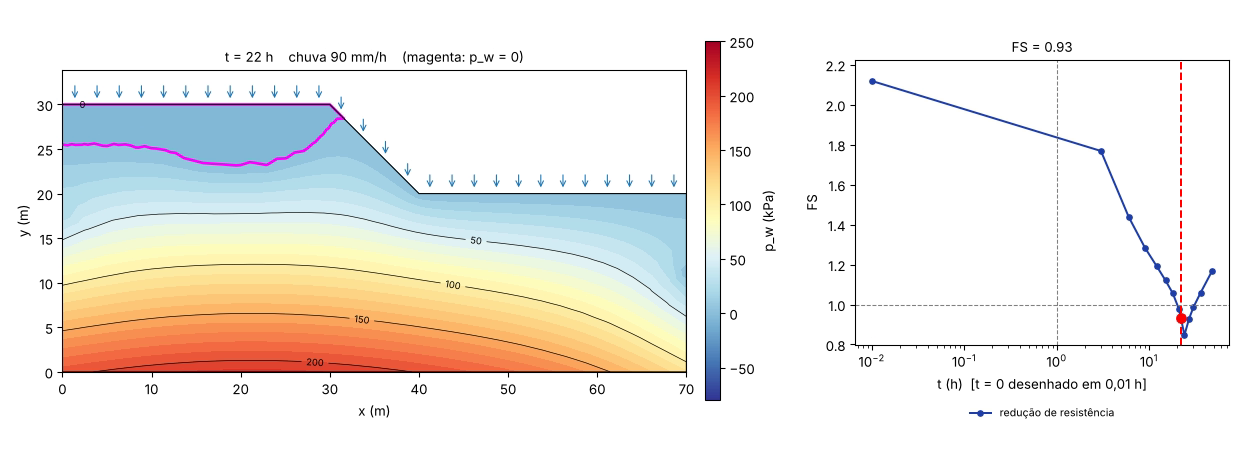
\includegraphics[width=0.50\textwidth]{figuras/quadro_animacao_f50_I90.png}
\caption{Esquerda: FS($t$) em escala log, modelo completo, $f_{50,-5}$, 36~mm/h (SRM e GI). Direita: quadro da
anima\c{c}\~ao (desacoplado, 90~mm/h, $t=22$~h).}\label{fig:fstempo}
\end{figure}

%======================================================================
\section{Contraexemplos \`as conclus\~oes de Rahardjo et al.\ (2007)}\label{sec:contraexemplos}
%======================================================================

As conclus\~oes do artigo foram obtidas com percola\c{c}\~ao desacoplada, ar passivo, solo isotr\'opico, $\chi=1$,
suc\c{c}\~ao inicial limitada a 75~kPa e equil\'ibrio-limite com superf\'icies circulares. O modelo desta nota permite
relaxar cada uma dessas hip\'oteses. Os itens abaixo s\~ao hip\'oteses de investiga\c{c}\~ao que podem contradizer
(ou restringir) as conclus\~oes do artigo; para cada um indicam-se a evid\^encia j\'a obtida e o teste proposto.

\subsection{A1. O patamar de FS m\'inimo (``intensidade-limite'') depende da dilat\^ancia}

\textbf{Conclus\~ao do artigo:} existe uma intensidade $I_{r(\mathrm{thr})}$ acima da qual o FS m\'inimo n\~ao diminui,
com patamar inferior 0,81--0,82 (Eq.~6, Fig.~7).

\textbf{Evid\^encia:} desacoplado, o NeoPZ reproduz o patamar (0,84--0,86); acoplado, o patamar sobe para
$\approx1{,}00$ e o transiente nunca perde o equil\'ibrio (Tabela~\ref{tab:B}). O mecanismo proposto \'e a suc\c{c}\~ao
gerada pela dilat\^ancia pl\'astica ($\psi=\phi'$) na percola\c{c}\~ao acoplada.

\textbf{Teste:} repetir a S\'erie B acoplada com $\psi=0$, $\phi'/2$ e $\phi'$. Se o patamar descer de 1,00 a 0,82
quando $\psi\to0$, a ``intensidade-limite com FS $<1$'' depende de uma hip\'otese constitutiva n\~ao discutida no
artigo, e a an\'alise desacoplada \'e conservadora apenas para solos contrativos. \emph{Requer} um Mohr--Coulomb
n\~ao associativo (o retorno anal\'itico atual exige $\psi=\phi'$; alternativa: \texttt{TPZPlasticStepPV}).

\subsection{A2. ``Taludes pouco perme\'aveis s\~ao seguros em chuvas curtas''}

\textbf{Conclus\~ao do artigo:} solos com $k_s\le10^{-6}$~m/s n\~ao rompem em chuvas de at\'e 24~h, qualquer que seja a
intensidade (categoria IV, sem eleva\c{c}\~ao do NA).

\textbf{Evid\^encia:} com ar ativo o FS m\'inimo do $f_{100}$ cai de 1,50 (ar passivo) para 1,28 com 18~mm/h e
de 1,48 para 1,28 com 36~mm/h (Tabela~\ref{tab:B}), ficando abaixo da Eq.~6 (1,45); o ar aprisionado chega a
50~kPa e torna $p_w$ positiva sob a frente (Fig.~\ref{fig:campos}). Na S\'erie A, com ar ativo, o $f_{100}$ com
80~mm/h chega a 1,01 em $\alpha=63{,}4^\circ$.

\textbf{Teste:} $f_{100}$ com $\alpha=63{,}4^\circ$ e $H_s=20$~m, chuvas de 9 a 80~mm/h, com e sem ar ativo, e
$k_{ra}^{\min}$ variando de $10^{-6}$ a $10^{-2}$ (a sa\'ida do ar controla a pressuriza\c{c}\~ao). Um FS $<1$ apenas
com ar ativo seria um contraexemplo direto. N\~ao requer c\'odigo novo.

\subsection{A3. ``O controle \'e $k_s$'': com anisotropia $k_s$ n\~ao \'e um n\'umero}

\textbf{Conclus\~ao do artigo:} $I_{r(\mathrm{ini})}$ e $I_{r(\mathrm{thr})}$ s\~ao dados em m\'ultiplos de $k_s$
($0{,}03$--$0{,}78k_s$ e $0{,}39$--$3k_s$, Fig.~7).

\textbf{Evid\^encia:} mesmo solo, mesma chuva e o mesmo $k_{\min}$, s\'o girando o tensor: FS m\'inimo de 1,08 a 1,33
(Tabela~\ref{tab:rot}); com $k_x/k_y=10$, FS de 1,08 ou 1,26 conforme qual componente vale $k_s$.

\textbf{Teste:} curvas FS m\'inimo $\times$ $I_r$ (S\'erie B) para $k_1/k_2=10$ e $\theta=0$, $45^\circ$ e $135^\circ$,
verificando se a sigmoide se desloca com $k_y$, com a condutividade normal \`a superf\'icie, com a condutividade ao
longo da face ou com $\sqrt{k_1k_2}$. N\~ao requer c\'odigo novo ($\approx20$ casos).

\subsection{A4. ``O len\c{c}ol fre\'atico inicial \'e secund\'ario'': efeito do limite de suc\c{c}\~ao}

\textbf{Conclus\~ao do artigo:} $H_w$ s\'o define o FS inicial; o pr\'oprio artigo nota que o FS inicial deixa de
crescer acima de $H_w=7{,}5$~m por causa do limite de $-75$~kPa (Fig.~8).

\textbf{Teste:} S\'erie C com suc\c{c}\~ao inicial limitada a 75, 150 e 300~kPa e sem limite. Se a queda de FS
(FS inicial $-$ FS m\'inimo) passar a depender fortemente de $H_w$, o car\'ater ``secund\'ario'' do NA \'e artefato do
limite. \emph{Requer} tornar o limite (\texttt{SMAX}) um par\^ametro.

\subsection{A5. ``O FS m\'inimo \'e linear em $\alpha$ com inclina\c{c}\~ao quase constante''}

\textbf{Conclus\~ao do artigo:} $F_{s(\min)}=E+F\alpha$ com $F\approx-0{,}025$ (Tabela~7).

\textbf{Evid\^encia:} a Tabela~7 n\~ao reproduz a Fig.~9 em algumas linhas; com quatro \^angulos a linearidade n\~ao
\'e test\'avel. No NeoPZ a inclina\c{c}\~ao muda nas chuvas fortes por causa do patamar $\approx1$.

\textbf{Teste:} $\alpha$ de $20^\circ$ a $70^\circ$ a cada $5^\circ$ para os nove pares solo--chuva, observando
tamb\'em a profundidade do mecanismo (zona pl\'astica rasa $\times$ profunda). N\~ao requer c\'odigo novo.

\subsection{A6. Intensidade ou volume?}

\textbf{Conclus\~ao do artigo:} $I_r=1k_s$ n\~ao produz necessariamente o menor FS; o volume $V_r$ \'e citado, mas
todas as chuvas t\^em 24~h.

\textbf{Teste:} chuvas com o mesmo volume e dura\c{c}\~oes de 3, 6, 24 e 72~h. Se o FS m\'inimo depender s\'o do volume
para solos de alto $k_s$ e s\'o da intensidade para solos de baixo $k_s$, a conclus\~ao precisa ser reformulada. N\~ao
requer c\'odigo novo (par\^ametro \texttt{train}).

%======================================================================
\section{Novas dire\c{c}\~oes}\label{sec:direcoes}
%======================================================================

\subsection{B1. Defini\c{c}\~ao do fator de seguran\c{c}a com suc\c{c}\~ao}

O FS por aumento da gravidade \'e 5,7 contra 2,1 do SRM no estado inicial e varia muito mais com a orienta\c{c}\~ao do
tensor (1,24--2,21 contra 1,08--1,33). Proposta: comparar SRM, GI e Bishop simplificado nos mesmos campos de press\~ao
e verificar se o SRM detecta rupturas rasas na frente de umedecimento (transla\c{c}\~ao) que a superf\'icie circular de
Bishop n\~ao representa.

\subsection{B2. Par\^ametro de Bishop}

O artigo usa $\phi^b=\phi'$ ($\chi=1$). Com $\chi=S_w$ (j\'a dispon\'ivel no material) ou $\phi^b<\phi'$, a perda de
suc\c{c}\~ao pesa menos e o mecanismo atribu\'ido aos solos pouco perme\'aveis enfraquece; a tangente com
$\chi_w=S_w-\Gamma p_c$ (Se\c{c}\~ao 13.4) torna o acoplamento n\~ao sim\'etrico.

\subsection{B3. Chuva antecedente e padr\~ao temporal}

Duas chuvas separadas por intervalos secos e padr\~oes adiantado, atrasado e uniforme com o mesmo total. O artigo
afirma qualitativamente que a chuva antecedente importa para baixo $k_s$; no $f_{100}$ o m\'inimo j\'a ocorre depois
do fim da chuva ($t=27$~h). \emph{Requer} intensidade vari\'avel no tempo.

\subsection{B4. Tratamento da superf\'icie}

O artigo imp\~oe $q=I_r$; aqui a condi\c{c}\~ao \'e unilateral (escoamento superficial quando $p_w$ atinge 0). Rodar as
duas condi\c{c}\~oes isola quanto do patamar e da intensidade-limite vem do tratamento da superf\'icie.

\subsection{B5. F\'isica prevista na formula\c{c}\~ao e ainda n\~ao usada}

\begin{itemize}
\item histerese da curva de reten\c{c}\~ao (secagem $\times$ umedecimento), que deve afetar a recupera\c{c}\~ao depois da
chuva;
\item porosidade vari\'avel (Se\c{c}\~ao 9) e reten\c{c}\~ao dependente da porosidade (Se\c{c}\~ao 11) com
Kozeny--Carman;
\item evapora\c{c}\~ao e transpira\c{c}\~ao como fluxo negativo (Fig.~1 do artigo);
\item varia\c{c}\~ao espacial de $k_s$ e $c'$ (campos aleat\'orios), na linha de Ceron et al.\ (2025).
\end{itemize}

\subsection{Prioridades}

\begin{enumerate}
\item A2 (ar ativo em solo pouco perme\'avel): contraexemplo mais direto, sem c\'odigo novo.
\item A3 (anisotropia na sigmoide de $I_r$): usa o que foi implementado e pode gerar um resultado original.
\item A1 (dilat\^ancia): explica a diferen\c{c}a entre o modelo acoplado e o artigo; requer Mohr--Coulomb n\~ao
associativo.
\end{enumerate}

\subsection{Limita\c{c}\~oes dos resultados atuais}

\begin{itemize}
\item Em dois casos acoplados um passo n\~ao converge nem com 5 bissec\c{c}\~oes (FS $\approx1{,}8$--$1{,}9$); o instante \'e
registrado como ``transiente sem converg\^encia'', n\~ao como ruptura.
\item Na variante desacoplada, $f_{10}$ com 360 e 900~mm/h: a percola\c{c}\~ao parou de convergir \`as 8,5~h com toda a
superf\'icie alagada; o m\'inimo est\'a superestimado.
\item FS por elementos finitos (SRM) e n\~ao por equil\'ibrio-limite; porosidade constante; sem histerese; uma \'unica
malha (sem estudo de converg\^encia).
\end{itemize}


\section*{Refer\^encias para as rela\c{c}\~oes constitutivas}

\begin{itemize}
\item Lo et al. (2014), \emph{Poroelastic Theory of Consolidation in Unsaturated Soils},
\emph{Vadose Zone Journal}, DOI: \href{https://doi.org/10.2136/vzj2013.07.0117}{10.2136/vzj2013.07.0117}.
\item Mualem (1976), \emph{A New Model for Predicting the Hydraulic Conductivity of Unsaturated Porous Media},
\emph{Water Resources Research}, DOI: \href{https://doi.org/10.1029/WR012i003p00513}{10.1029/WR012i003p00513}.
\item Rela\c{c}\~oes de reten\c{c}\~ao e permeabilidade relativa:
\href{https://documentation.pflotran.org/theory_guide/constitutive_relations.html}{PFLOTRAN, Constitutive Relations}.
\item Fredlund e Rahardjo (1993), \emph{Soil Mechanics for Unsaturated Soils},
Cap\'itulo 16, exemplo de escoamento transiente em barragem de terra.
\item Rahardjo, Ong, Rezaur e Leong (2007), \emph{Factors controlling instability of homogeneous soil slopes under
rainfall}, \emph{J.\ Geotech.\ Geoenviron.\ Eng.} 133(12):1532--1543,
DOI: \href{https://doi.org/10.1061/(ASCE)1090-0241(2007)133:12(1532)}{10.1061/(ASCE)1090-0241(2007)133:12(1532)}.
\item Fredlund e Xing (1994), \emph{Equations for the soil-water characteristic curve}, \emph{Can.\ Geotech.\ J.}
31:521--532.
\item Leong e Rahardjo (1997), \emph{Permeability functions for unsaturated soils}, \emph{J.\ Geotech.\
Geoenviron.\ Eng.} 123(12):1118--1126.
\item Fredlund, Morgenstern e Widger (1978), \emph{The shear strength of unsaturated soils}, \emph{Can.\ Geotech.\
J.} 15(3):313--321.
\item Ceron, Cec\'ilio, Linn e Maghous (2025), \emph{Stability analysis of slope subjected to seepage forces
considering spatial variability of soil properties}, \emph{Int.\ J.\ Numer.\ Anal.\ Methods Geomech.} 49(11).
\end{itemize}

\end{document}
